% %%%%%%%%%%%%%%%%%%%%%%%%%%%%%%%%%%%%%%%%%%%%%%%%%%%%%%%%%%%%%%%%%%%%%%%%%%%%%
% thesis.tex: Primary TeX control file for thesis.
% %%%%%%%%%%%%%%%%%%%%%%%%%%%%%%%%%%%%%%%%%%%%%%%%%%%%%%%%%%%%%%%%%%%%%%%%%%%%%
\documentclass[11pt, oneside]{mnthesis}
\usepackage{epsfig} % Allows the inclusion of eps files
\usepackage{epic} % Enhanced picture mode
\usepackage{eepic} % Extensions for epic
\usepackage{units} % SI unit typesetting
\usepackage{url} % URL handling
\usepackage{longtable} % Tables that continue onto multiple pages
\usepackage{mathrsfs} % Support for \mathscr script
\usepackage{multirow} % Span rows in tables
\usepackage{bigstrut} % Space struts in tables up and down
\usepackage{amssymb} % AMS math symbols and helpers
\usepackage{graphicx} % Enhanced graphics support
\usepackage{setspace} % Adjust spacing in captions, single by default
\usepackage{xspace} % Automatically adjusting space after macros
\usepackage{amsmath} % \text, and other math formatting options
\usepackage{siunitx} % \num{} formatting and SI unit formatting
\usepackage{booktabs} % Enhanced tables with \toprule, etc.
\usepackage{hyperref} % Add clickable links to other parts of the document
\usepackage[noabbrev,capitalize]{cleveref} % Automatically determine \cref type

\usepackage[hang,flushmargin]{footmisc} % Prevent indent in footnotes. 

% Put captions tighter to their figures. Not clear if it actually works. 
\setlength{\abovecaptionskip}{0pt}

\usepackage{xcolor} % so we can put todo notes in color. 

\usepackage{doi} % Link to doi in the bibliography. Doesn't seem to work. 

\usepackage{parskip} % http://ctan.org/pkg/parskip vskip instead of indent. 

\usepackage{float} % Sometimes you want to tell LaTeX to put an image RIGHT HERE. 


% Configure the siunitx package
\sisetup{
    group-separator = {,}, % Use , to separate groups of digits, like 12,345
    list-final-separator = {, and } % Always use the serial comma in \SIlist
}

% Configure the cleveref package
\newcommand{\creflastconjunction}{, and } % Always use the serial comma




% Names with special characters. 
\newcommand{\Alfven}{Alfv\'en\xspace}
\newcommand{\Ampere}{Amp\`ere\xspace}

% To make sure the capitalization is consistent. 
\newcommand{\ohmlaw}{Ohm's Law\xspace}
\newcommand{\amplaw}{\Ampere's Law\xspace}
\newcommand{\farlaw}{Faraday's Law\xspace}

% Field-aligned unit vectors. 
\newcommand{\xhat}{\ensuremath{\hat{x}}\xspace}
\newcommand{\yhat}{\ensuremath{\hat{y}}\xspace}
\newcommand{\zhat}{\ensuremath{\hat{z}}\xspace}

% Spherical unit vectors. 
\newcommand{\rhat}{\ensuremath{\hat{r}}\xspace}
\newcommand{\qhat}{\ensuremath{\hat{\theta}}\xspace}
\newcommand{\fhat}{\ensuremath{\hat{\phi}}\xspace}

% Use underlines for vectors and tensors. 
\renewcommand{\vec}[1]{\underline{#1}}
\newcommand{\tensor}[1]{\underline{\underline{#1}}}

% Differential operators. 
\newcommand{\dd}[1]{\ensuremath{ \frac{\partial}{\partial #1} }\xspace}
\newcommand{\ddt}{\dd{t}\xspace}
\newcommand{\curl}[1]{\ensuremath{ \nabla \times \vec{#1} }\xspace}
\renewcommand{\div}[1]{\ensuremath{ \nabla \cdot \vec{#1} }\xspace}
\newcommand{\grad}[1]{\ensuremath{ \nabla #1 }\xspace}

% Properly-scaled parentheses for grouping terms or for arguments. 
\newcommand{\lr}[1]{ \left( #1 \right) }
\newcommand{\lrsmall}[1]{ \left( {\scriptstyle #1} \right) }
\renewcommand{\arg}[1]{\!\lr{#1}}
\newcommand{\argsmall}[1]{\!\lrsmall{#1}}
\newcommand{\lrb}[1]{ \left[ #1 \right] }

% Circled plus-minus symbol. Solving quartics requires \pm and \opm. 
\newcommand{\opm}{ \text{ \textcircled{ \ensuremath{\hskip -0.2em \pm} } } \xspace}

% Define a better looking eV by moving the V slightly left
\DeclareSIUnit\electronvolt{e\hspace{-0.08em}V}

\DeclareSIUnit\RE{R_E}


\newcommand{\dt}{\ensuremath{\delta \hspace{-0.1em} t} \xspace}



% Azimuthal modenumber, typically indicated with a lowercase m. 
\newcommand{\azm}{\ensuremath{m_{azimuthal}}\xspace}

% Azimuthal modenumber, typically indicated with a lowercase m. 
\newcommand{\me}{\ensuremath{m_{e}}\xspace}

% Jacobian dererminant, typically indicated with a capital J, which we are using for current. 
\newcommand{\jac}{\ensuremath{D}\xspace}

% Dispersion tensor, typically indicated with... a capital D?
\newcommand{\dispersiontensor}{\tensor{T}\xspace}


% These things just get used a lot in the dispersion relation chapter...

% Boris-corrected speed of light. 
\newcommand{\cb}{\ensuremath{c_B} \xspace}

% Boris-corrected plasma frequency. 
\newcommand{\ob}{\ensuremath{\omega_B} \xspace}

% Boris-corrected electric constant. 
\newcommand{\eb}{\ensuremath{\epsilon_B} \xspace}

% Alfven speed. 
\newcommand{\va}{\ensuremath{v_A} \xspace}

% Perpendicular electric constant. 
\newcommand{\ep}{\ensuremath{\epsilon_\bot} \xspace}

% Epsilon zero. 
\newcommand{\ez}{\ensuremath{\epsilon_0} \xspace}

% Conductivities. 
\newcommand{\sz}{\ensuremath{\sigma_0} \xspace}
\newcommand{\sh}{\ensuremath{\sigma_H} \xspace}
\renewcommand{\sp}{\ensuremath{\sigma_P} \xspace}




\newcommand{\spe}{\ensuremath{\frac{\sigma_P}{\ep}} \xspace}
\newcommand{\she}{\ensuremath{\frac{\sigma_H}{\ep}} \xspace}




% 3x3 matrix. 
\newcommand{\mmm}[9]{ \left[ \begin{array}{ccc}
    #1 & #2 & #3 \\
    #4 & #5 & #6 \\
    #7 & #8 & #9
  \end{array} \right] }

% 2x2 matrix. 
\newcommand{\mm}[4]{ \left[ \begin{array}{cc}
    #1 & #2 \\
    #3 & #4
  \end{array} \right] }

% 2x1 matrix, or 2-vector. 
\newcommand{\vv}[2]{ \left[ \begin{array}{c}
    #1 \\
    #2
  \end{array} \right] }


% Physics constants
\newcommand{\C}{{\mathrm{c}}}

% Add space between rows of tables
\newcommand{\spacerows}[1]{\renewcommand{\arraystretch}{#1}}









\linespread{1.3}

% Compile only the chapters listed here. This may make the compile faster, but
% it's not necessary. 
%\includeonly{
%    preliminaries/title,
%    chapters/intro,
%    chapters/model,
%    chapters/math,
%    chapters/results,
%    chapters/data,
%    chapters/conclusion,
%    chapters/app_geometry,
%    chapters/app_integrating,
%}



% %%%%%%%%%%%%%%%%%%%%%%%%%%%%%%%%%%%%%%%%%%%%%%%%%%%%%%%%%%%%%%%%%%%%%%%%%%%%%
% %%%%%%%%%%%%%%%%%%%%%%%%%%%%%%%%%%%%%%%%%%%%%%%%%%%%%%% Mark this as a draft. 
% %%%%%%%%%%%%%%%%%%%%%%%%%%%%%%%%%%%%%%%%%%%%%%%%%%%%%%%%%%%%%%%%%%%%%%%%%%%%%
\draft
% %%%%%%%%%%%%%%%%%%%%%%%%%%%%%%%%%%%%%%%%%%%%%%%%%%%%%%%%%%%%%%%%%%%%%%%%%%%%%
% %%%%%%%%%%%%%%%%%%%%%%%%%%%%%%%%%%%%%%%%%%%%%%%%%%%%%%%%%%%%%%%%%%%%%%%%%%%%%
% %%%%%%%%%%%%%%%%%%%%%%%%%%%%%%%%%%%%%%%%%%%%%%%%%%%%%%%%%%%%%%%%%%%%%%%%%%%%%



\begin{document}
%\bibliographystyle{hunsrt} % style of bibliography
\bibliographystyle{abbrv} % style of bibliography

% Title and other sections that come before the body of the document
%%%%%%%%%%%%%%%%%%%%%%%%%%%%%%%%%%%%%%%%%%%%%%%%%%%%%%%%%%%%%%%%%%%%%%%%%%%%%%%%
% title.tex - Set up the beginning of thesis.
%%%%%%%%%%%%%%%%%%%%%%%%%%%%%%%%%%%%%%%%%%%%%%%%%%%%%%%%%%%%%%%%%%%%%%%%%%%%%%%%

% Uncomment to turn on draft mode, which changes the title page to have a draft
% label and date of compilation
%\draft

% Set the type of thesis
\phd % use if for a Ph.D. dissertation
%\ms % use if for a Master of Science thesis

% Set the title and your name. Remember that the guidelines state:
%
% "The title of the thesis must not contain chemical or mathematical formulas,
% symbols, superscripts, subscripts, Greek letters, or other non-standard
% characters; words must be substituted."
\title{\bf Modeling Current-Driven Pc4 Pulsations in Two and a Half Dimensions}
\author{Charles A McEachern}
% Advisor name, put co-advisors here as well separated by commas
\director{Robert L Lysak}

% Specify the month and year; if commented out then these default to the
% current month and year
\submissionmonth{April}
\submissionyear{2016}

% Pages after the title page
\abstract{% %%%%%%%%%%%%%%%%%%%%%%%%%%%%%%%%%%%%%%%%%%%%%%%%%%%%%%%%%%%%%%%%%%%%%%%%%%%%%
% %%%%%%%%%%%%%%%%%%%%%%%%%%%%%%%%%%%%%%%%%%%%%%%%%%%%%%%%%%%%%%%%%%%% Abstract
% %%%%%%%%%%%%%%%%%%%%%%%%%%%%%%%%%%%%%%%%%%%%%%%%%%%%%%%%%%%%%%%%%%%%%%%%%%%%%

Abstract placeholder. 
}
\copyrightpage % Do you want copyright protection?
\acknowledgements{%%%%%%%%%%%%%%%%%%%%%%%%%%%%%%%%%%%%%%%%%%%%%%%%%%%%%%%%%%%%%%%%%%%%%%%%%%%%%%%%
% acknowledge.tex: Acknowledgements
%%%%%%%%%%%%%%%%%%%%%%%%%%%%%%%%%%%%%%%%%%%%%%%%%%%%%%%%%%%%%%%%%%%%%%%%%%%%%%%%

There are many people that have earned my gratitude for their contribution to my
time in graduate school.

%%%%%%%%%%%%%%%%%%%%%%%%%%%%%%%%%%%%%%%%%%%%%%%%%%%%%%%%%%%%%%%%%%%%%%%%%%%%%%%%
}
\dedication{% %%%%%%%%%%%%%%%%%%%%%%%%%%%%%%%%%%%%%%%%%%%%%%%%%%%%%%%%%%%%%%%%%%%%%%%%%%%%%
% %%%%%%%%%%%%%%%%%%%%%%%%%%%%%%%%%%%%%%%%%%%%%%%%%%%%%%%%%%%%%%%%%% Dedication
% %%%%%%%%%%%%%%%%%%%%%%%%%%%%%%%%%%%%%%%%%%%%%%%%%%%%%%%%%%%%%%%%%%%%%%%%%%%%%

\todo{$\cdots$}

}

% Use a special preface
%\extra{\input{preface}}

% The \beforepreface command actually causes insertion of the title,
% abstract, signature, and copyright pages into the new document.
\beforepreface

% Define the text to go before the table of contents
\figurespage
\tablespage

% The \afterpreface command actually causes insertion of the
% contents, list of figures, etc. into the new document.
\afterpreface
%%%%%%%%%%%%%%%%%%%%%%%%%%%%%%%%%%%%%%%%%%%%%%%%%%%%%%%%%%%%%%%%%%%%%%%%%%%%%%%%





\chapter{Introduction}
  \label{ch_intro}

%ALEX NOTES: 
%- Should decide if you're going to use contractions or not; many would say not to in formal writing

\todo{In 1859, humanity was working hard to get its shit together.} The United States moved steadily toward the American Civil War, which would abolish slavery and consolidate the power of the federal government. A slew of conflicts in Southern Europe, such as the Austro-Sardinian War, set the stage for the unification of Italy. The Taiping Civil War --- one of the bloodiest conflicts of all time --- is considered by many to mark the beginning of modern Chinese history. Origin of Species was published. The first transatlantic telegraph cable was laid.

Meanwhile, ambivalent to humanity, the Sun belched an intense burst of charged particles and magnetic energy directly at Earth. The resulting geomagnetic storm\footnote{The Solar Storm of 1859 is also called the Carrington Event, after English astronomer Richard Carrington. He drew a connection between the storm's geomagnetic activity and the sunspots he had observed the day before.} caused telegraph systems to fail across the Western hemisphere, electrocuting operators and starting fires\cite{green_2006,tsurutani_2003}. Displays of the northern lights were visible as far south as Cuba. 

The Solar Storm of 1859 was perhaps the most powerful in recorded history, but by no means was it a one-time event. The Sun discharges hundreds of coronal mass ejections (CMEs) per year, of all sizes, in all directions. In fact, a comparably large CME narrowly missed Earth in 2012\cite{nasa_2012}. Had it not, it's estimated it would have caused widespread, long-term electrical outages, with a damage toll on the order of \num{e12} dollars\cite{lloyds_2013}. 

The Sun's extreme --- and temperamental --- effect on Earth's magnetic environment makes a compelling case for the ongoing study of space weather. Such research has evolved over the past century from sunspot counts and compass readings to multi-satellite missions and supercomputer simulations. Modern methods have dramatically increased humanity's understanding of the relationship between the Sun and the Earth; however, significant uncertainty continues to surround geomagnetic storms, substorms, and the various energy transport mechanisms that make them up. 

The present work focuses in particular on the phenomenon of field line resonance: \Alfven waves bouncing between the northern and southern hemispheres. Such waves play an important part in the energization of magnetospheric particles, the transport of energy from high to low altitude, and the driving of currents at the top of the atmosphere. 

\section{Structure of the Present Work}

\cref{ch_environment} surveys the near-Earth environment. Prominent features of the magnetosphere are defined. The response of the magnetosphere to transient solar wind events is summarized. 

\cref{ch_flrs} introduces the field line resonance phenomenon, in terms of both the underlying physics and notable work on the topic. Jargon is introduced to clarify important elements of wave structure. Several open questions about field line resonances (FLRs) are offered as motivations for the present work. 

\cref{ch_math} lays the groundwork for a numerical model by exploring the fundamental equations of waves in a cold, resistive plasma --- such as Earth's magnetosphere. Characteristic scales are gleaned from the resulting dispersion relations. 

\cref{ch_model} presents Tuna, a new two and a half dimensional simulation designed specifically for the realistic modeling of FLRs. Tuna's non-orthogonal geometry, height-resolved ionosphere, novel driving mechanism, and coupling to the atmosphere are explained. 

\cref{ch_inertia} considers the addition of electron inertial effects to Tuna, touches on what can be learned from them, and shows that they incur an unreasonable computational cost. (Electron inertia is neglected in the results presented in other chapters.)

\cref{ch_results} describes the core numerical results of the work, unifying several of the questions posed in \cref{ch_flrs}. Significant depth is added to past work on finite poloidal lifetimes\cite{mann_1995,radoski_1974}. Interplay between poloidal-toroidal coupling, shear-compressional coupling, and Joule dissipation is considered from several angles. 

\cref{ch_rbsp} puts the numerical results in physical context through the analysis of data from the Van Allen Probes mission. FLR occurrence rates are considered in terms of not only location, but mode structure and polarization as well --- parameters which are not considered in other recent FLR surveys\cite{dai_2015,motoba_2015}. 

\cref{ch_conclusion} briefly summarizes the results shown in the above chapters --- the code development, analysis of numerical results, and satellite observation --- and suggests further directions. 

%\todo{The storm of 1859 presented compelling evidence that the Sun drives geomagnetic activity. In the decades that followed, a model took shape to describe the mechanisms of energy transfer between the Sun and the Earth. Based on auroral observations and data from ground-based magnetometers, Birkeland argued for the existence of a constant outflow of electrons and ions from the Sun -- the solar wind. The advent of high-frequency radio communication allowed Kennelly, Heaviside, and others to probe the electrical properties of the upper atmosphere. }

%\todo{The study of space weather was revolutionized by the development of sounding rockets and satellites in the mid twentieth century. This allowed direct observation of the structure of the near-Earth environment, including, crucially, the waves that carry energy through it. }

%\todo{Not least among these advances was the discovery of \Alfven waves. {\Alfven}ic aurora. Carry energy and particles. }

%The study of space weather revolves around the transfer of energy from the Sun to the Earth. Ultra low frequency waves in particular are an important energy transport mechanism between the magnetosphere's outer boundary (at the solar wind) and its inner boundary (at the top of the atmosphere). 

%\footnote{Uppercase \X, \Y, and \Z are used to indicate GSE coordinates: \Xhat points from the Earth to the Sun; \Yhat is perpendicular to \Xhat in the Sun's ecliptic plane, pointing duskwards; \Zhat points north, out of the ecliptic plane. In later chapters, lowercase \x, \y, and \z are used to define a more or less analogous corodinate system with respect to Earth. }

% The moon is at \SI{60}{\RE}. 

% Transient solar wind phenomena, such as coronal mass ejections, are also known to be related to geomagnetic disturbances at Earth. Jesse cites here: 

% R. L. McPherron. Physical processes producing magnetospheric substorms and mangetic storms. In J. A. Jacobs, editor, Geomagnetism, volume 4, chapter 7. Academic Press, 1991.

% G. Rostoker. Substorms. In Handbook of the Solar-Terrestrial Environment, chapter 15. Springer-Verlag, 2007.

% M. Shulz. Magnetospheres. In Handbook of the Solar-Terrestrial Environment, chapter 7. Springer-Verlag, 2007.

% papers mentioned during Yan's talk. mostly about alfven acceleration and nonlinear effects. 
% Vasyliunas 1970, 1984
% Hasegawa 1976
% Goertz 1991
% Stasiewicz et al 2000
% Haerendel 2008
% Song & Lysak 1994, 1999, 2000, 2001, 2006, 2011, 2012
% Inverted V?
% Double layers? 
% Charge holes? 



% %%%%%%%%%%%%%%%%%%%%%%%%%%%%%%%%%%%%%%%%%%%%%%%%%%%%%%%%%%%%%%%%%%%%%%%%%%%%%
% %%%%%%%%%%%%%%%%%%%%%%%%%%%%%%%%%%%%%%%%%%%%%% Introduction to Pc4 Pulsations
% %%%%%%%%%%%%%%%%%%%%%%%%%%%%%%%%%%%%%%%%%%%%%%%%%%%%%%%%%%%%%%%%%%%%%%%%%%%%%

\chapter{Ultra Low Frequency Waves}
  \label{ch_waves}




% %%%%%%%%%%%%%%%%%%%%%%%%%%%%%%%%%%%%%%%%%%%%%%%%%%%%%%%%%%%%%%%%%%%%%%%%%%%%%
% %%%%%%%%%%%%%%%%%%%%%%%%%%%%%%%%%%%%%%%%%%%%%% Description of Numerical Model
% %%%%%%%%%%%%%%%%%%%%%%%%%%%%%%%%%%%%%%%%%%%%%%%%%%%%%%%%%%%%%%%%%%%%%%%%%%%%%

\chapter{Numerical Model}
\label{ch_model}

The model works in two and a half dimensions. A meridional slice of the magnetosphere is resolved. Fields are presumed to vary azimuthally according to a fixed modenumber \azm. Derivatives in $\phi$ are replaced by $i \azm$. Imaginary field values indicate a phase shift in the azimuthal direction. 

\todo{Note that Lysak's 2013 paper\cite{lysak_2013} was 2.5D. }

The use of a fixed modenumber allows a dramatic decrease in computational cost. Waves with very high azimuthal modenumber are prohibitively expensive to simulate since they can only be resolved if grid resolution is very fine in the azimuthal direction. 

\todo{Has anyone actually talked about computational expense as a constraint on high-\azm simulations?}

This prevents the simultaneous consideration of dayside and nightside phenomena, but is fine for azimuthally-localized waves. As was shown by \cite{engebretson_1987}, and recently confirmed in detail by \cite{dai_2015}, Pc4 pulsations are generally confined to just a few hours MLT on the dayside. 

Driving with a compressional pulse from the outer boundary of a simulation is typical. This model also includes a novel driving mechanism: perturbations to the ring current. 

The code is linear. All magnetic fields are a first-order perturbation over the zeroth-order dipole field. This is a not-great assumption out towards the magnetopause. In practice, however, most activity is within $L \sim \SI{7}{\RE}$, where the dipole approximation is pretty good. 

Models with height-resolved ionospheres are a very recent development. Lysak presented his in 2013\cite{lysak_2013}. 

Ground signatures are fairly recent as well. 

\todo{Some ground signature work as far back as Greifinger and Greifinger in 1968, but there's been steady advancement. Lysak and Song, in 2006, were the first to work out ground signatures without the assumption of a single-frequency wave. }

\todo{The support software -- the driver and the plotter -- are significant too. Do they go in a section? In an appendix? }

\todo{Past FLR simulations focused on a single mode, didn't account well for the ionosphere, etc. Lee and Lysak 1989, 1990, 1991, Rankin et al 1993, 1995, 1999, Tikhonchuk and Rankin 2000, 2002. }

\todo{Past work that got ground signatures (without latitude-dependent zenith angle) Greifinger and Greifinger 1968, 1973, Hughes 1974, Sciffer and Waters 2002, Sciffer et al 2005. Better computation of ground signatures... Waters and Sciffer 2008, Sciffer and Waters 2011, Woodroffe and Lysak 2012. }

Note that the model uses \si{\mega\meter}, \si{\second}, \si{\mega\coulomb}, and \si{\gram} as the fundamental units of length, time, charge, and mass respectively. As a result, electric field is measured in \si{\mV/\meter}, magnetic field is measured in \si{\nano\tesla}, and Poynting flux is measured in \si{\mW/\meter\squared}. 



% =============================================================================
% =============================================================================
% =============================================================================
\section{Coordinate System}
  \label{sec_coords}

When referring to fields in place, it's convenient to use lowercase\footnote{ Not to be confused with uppercase \X, \Y, and \Z, which orient relative to the sun; see \cref{ch_intro} } \x, \y, and \z in their usual dipolar sense. The unit vector \zhat is aligned with the dipole field (pointing outward in the northern hemisphere and inward in the southern hemisphere), while \xhat is perpendicular to \zhat within the meridional plane and \yhat points in the azimuthal direction. 

\todo{Double-check the signs for \x (radially inward or outward at the equator?) and \y (east or west?). }

\todo{Wait... are \x, \y, and \z the same as Radoski's coordinates? }

It's convenient to align the grid with the zeroth-order magnetic field, which is presumed to be a perfect dipole. Field line resonances (such as Pc4 pulsations) are guided by magnetic field lines. 

\todo{Who showed that ULF waves can be guided? Cite them. }

A typical outermost field line has an equatorial radius of \SI{10}{\RE}. At this point, the ideal dipole approximation is suspect, particularly on the dayside. In practice, however, most wave activity is concentrated around $L \sim \num{7}$. 

\todo{Discuss, in Future Work, how the grid would be generalized. }

Radoski did theoretical work in the following dipole coordinates\cite{radoski_1967_coords}. 
\begin{align}
  \label{radoski_coords}
  \radx & = -\frac{\sin^2 \theta}{r} & \rady & = \phi & \radz & = \frac{\cos \theta}{r^2}
\end{align}

\todo{The symbol $\nu$ is overused. Reserve it for collision frequency. Use something else here. }

It's also convenient to take into account the effects of the ionosphere, the lower boundary of which is governed by gravity, and thus has a more-or-less constant altitude. If the above coordinates are used, no line of constant $\radz$ coincides with the ionosphere, at least not over a significant range of latitudes. 

Many previous works have used an effective ionosphere of nonuniform altitude. 

\todo{Figure out which previous works are worth citing here. Options include Radoski 1967, Lee and Lysak 1989, 1991, Rankin et al 1993, 1994, Streltsov and Lotko 1995, 1999. }


\todo{"The ionosphere is important for \Alfven waves." Cite this. }

In order to accommodate dipole field lines as well as a fixed-altitude ionosphere, a nonorthogonal grid is necessary. Such a grid was worked out numerically by Proehl\cite{proehl_2002}, then formalized analytically by Lysak\cite{lysak_2004}:
\begin{align}
  \label{def_coords}
  \lysakx & = - \frac{R_I}{r} \sin^2 \theta & 
  \lysaky & = \phi &
  \lysakz & = \frac{R_I^2}{r^2} \frac{\cos \theta}{\cos \theta_0}
\end{align}

The term $R_I$ indicates the ionosphere's position relative to Earth's center. It's generally taken to be \SI{1}{\RE} + \SI{100}{\km}. 

Like \radx and \rady, the coordinates \lysakx and \lysaky index a field line. However, compared to \radz, \lysakz has been renormalized by $\cos \theta_0$, where $\theta_0$ is the colatitude where each field line intersects the ionosphere in the northern hemisphere. As a result, for all field lines, $\lysakz = \pm 1$ at the northern and southern foot points. 

In terms of the McIlwain parameter, $\lysakx = -\frac{R_I}{L}$, and $\cos \theta_0 = \sqrt{ 1 - \frac{R_I}{L} }$

Compared to \cref{radoski_coords}, \cref{def_coords} represents a renormalization of indexing along each field line. The field lines themselves are not deformed. 

\todo{Explain how we set up the grid. It should only take a paragraph or two -- it doesn't need its own section. }

\todo{Plot of the grid setup! }

% -----------------------------------------------------------------------------
% -----------------------------------------------------------------------------
% -----------------------------------------------------------------------------
\subsection{Covariant and Contravariant Bases}
  \label{sec_basis}

The coordinates defined in \cref{def_coords} are not orthonormal. As a result, it's necessary to consider covariant and contravariant basis vectors separately. 

Covariant basis vectors $e_i \equiv \dd{\lysaki} \vec{x}$ are normal to the curve defined by constant $\lysaki$. 

Contravariant basis vectors $e^i \equiv \dd{ \vec{x} } \lysaki$ are tangent to the coordinate curve. Equally, they're normal to the plane defined by constant $\lysakj$ for all $j \ne i$. 

The basis vectors are reciprocal to one another\cite{dhaeseleer_1991}, and can be used to define the metric tensor $g$. 
\begin{align}
  \label{metric_basics}
  \hat{e}^i \cdot \hat{e}_j &= \delta^i_j & \hat{e}_i \cdot \hat{e}_j &= g_{ij} & \hat{e}^i \cdot \hat{e}^j &= g^{ij}
\end{align}

Note $\delta^i_j$ is the Kronecker delta, $\varepsilon^{ijk}$ is the Levi-Civita symbol, and summation is implied over repeated indeces per Einstein's convention\cite{einstein_1916}. 

The metric tensor is used to map between the covariant and contravariant representations of a vector
\begin{align}
  \label{metric_usage}
  A_i &= g_{ij} A^j & A^i &= g^{ij} A_j && \text{where} & A_i &\equiv \vec{A} \cdot \hat{e}_i &  A^i &\equiv \vec{A} \cdot \hat{e}^i
\end{align}

The Jacobian, used for mapping differential volume elements between bases, can be expressed as the square root of the determinant of the metric tensor. 
\begin{align}
  \label{def_jacobian}
  \jac &= \sqrt{ \varepsilon^{ijk} g_{1i} g_{2j} g_{3k} } && \text{where} & \jac d\lysakx d\lysaky d\lysakz &= dV
\end{align}

This quantity is also used when expressing a curl or cross product in generalized coordinates. 
\begin{align}
  \label{jacobian_usage}
  \lr{ \curl{A} }^i &= \frac{ \varepsilon^{ijk} }{\jac} \dd{\lysakj} A_k & \lr{ \cross{A}{B} }^i &= \frac{ \varepsilon^{ijk} }{\jac} A_j B_k
\end{align}

% -----------------------------------------------------------------------------
% -----------------------------------------------------------------------------
% -----------------------------------------------------------------------------
\subsection{Mapping to Physical Coordinates}

The full expression for the basis vectors, metric tensor, and Jacobian determinant discussed in \cref{sec_basis} can be found in the appendix of \cite{lysak_2004}. 

\todo{These expressions should probably be written out an in appendix here too...}

The basis vectors can be renormalized to produce unit vectors along the dipole coordinates \x, \y, and \z. 
\begin{align}
  \label{def_xyz_directions}
  \xhat &= \frac{1}{ \sqrt{ g^{11} } } \hat{e}^1 &
  \yhat &= \frac{1}{ \sqrt{ g^{22} } } \hat{e}^2 &
  \zhat &= \frac{1}{ \sqrt{ g_{33} } } \hat{e}_3
\end{align}

In addition, this coordinate system provides horizontal and radial unit vectors. Note that \cref{def_rqf_directions} is valid only at the ionospheric boundary. 
\begin{align}
  \label{def_rqf_directions}
  \qhat &= \frac{1}{ \sqrt{ g_{11} } } \hat{e}_1 &
  \fhat &= \frac{1}{ \sqrt{ g_{22} } } \hat{e}_2 &
  \rhat &= \frac{1}{ \sqrt{ g^{33} } } \hat{e}^3
\end{align}

% =============================================================================
% =============================================================================
% =============================================================================
\section{Ionospheric Profile}
  \label{sec_ionos}

The ionospheric profiles used in this model are based on values tabulated in the Appendix B of Kelley's book\cite{kelley_1989}. They were adapted by Lysak\cite{lysak_2013} to take into account the effect of the magnetosphere's latitude-dependent density profile. 

Mean molecular mass of \SI{28}{\amu} at \SI{100}{\km}, \SI{16}{\amu} around \SI{400}{\km}, down to \SI{1}{\amu} above \SI{1400}{\km}. 

Simulations are carried out using four profiles: active day, quiet day, active night, quiet night. 

Profiles are static for the duration of a simulation. Even so-called ultra low frequency waves are still much faster than convective timescales. 

\todo{Come up with a characteristic convective timescale or two, and cite it. }

% -----------------------------------------------------------------------------
% -----------------------------------------------------------------------------
% -----------------------------------------------------------------------------
\subsection{Conductivity}

The conductivity profiles used in this model are the tabulated values from \cite{kelley_1989}, rescaled by Lysak\cite{lysak_2013} to account for the increased mean molecular mass at low altitudes. 
\begin{align}
  \sp &= \displaystyle\sum_s \frac{n_s q_s^2}{m_s} \frac{\nu_s}{\nu_s^2 + \Omega_s^2} &
  \sh &= -\displaystyle\sum_s \frac{n_s q_s^2}{m_s} \frac{\Omega_s}{\nu_s^2 + \Omega_s^2} &
  \sz &= \displaystyle\sum_s \frac{n_s q_s^2}{m_s \nu_s}
\end{align}

Each profile is resolved to an altitude of about $\SI{1e4}{\km}$, and include well-resolved $E$, $F_1$, and $F_2$ layers. 

\todo{Talk about the ionospheric layers, probably in the introduction. }

\begin{figure}[H]
    \centering
    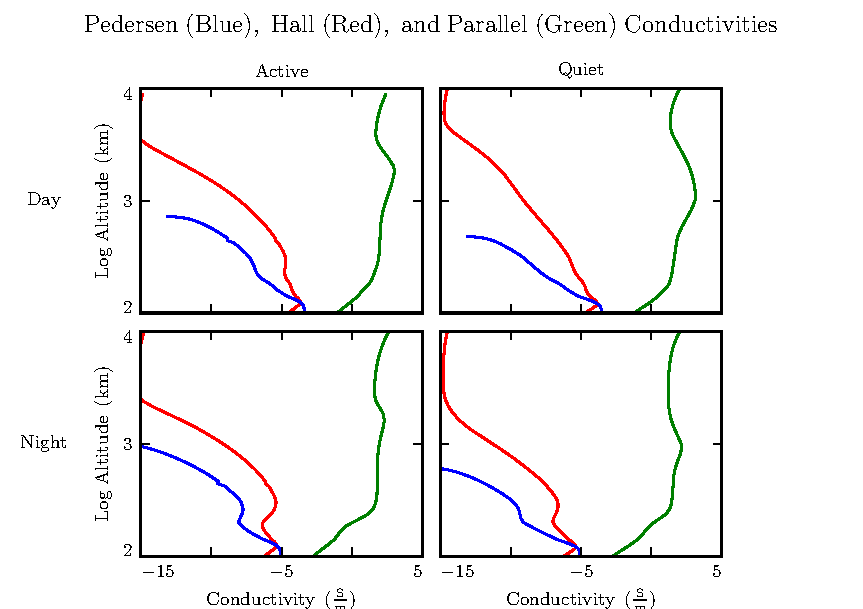
\includegraphics[width=\textwidth]{figures/sigma.pdf}
    \caption[Ionospheric Conductivity Profiles]{
      Ionospheric conductivity profiles, adapted by Lysak\cite{lysak_2013} from Appendix B of Kelley's textbook\cite{kelley_1989}. 
    }
    \label{fig_sigma}
\end{figure}

\todo{What is the height-interated conductivity for each profile? }

% -----------------------------------------------------------------------------
% -----------------------------------------------------------------------------
% -----------------------------------------------------------------------------
\subsection{\Alfven Speed}

The \Alfven speed is computed from Kelley's low-density profile, modified to take into account the local density. The density, in turn, is the sum of a plasmaspheric profile and a high-latitude auroral profile. 
\begin{align}
  \ep &= \text{(low-density tabulated value)} + \frac{ n \bar{m} }{B_0^2}
\end{align}

\todo{What's a clean way of showing the low-density \ep that we read in? }

\todo{Above the profile, Bob scales the value that's read in as $r^5$ or something. Is there a citation for that? }

Where $\bar{m}$ is the ambient mean molecular mass and $B_0$ is the zeroth-order magnetic field strength, $B_0 = \SI{3.11e4}{\nano\tesla} \lr{ \frac{R_E}{r} }^3 \sqrt{ 1 + 3 \cos^2 \theta }$. Note that \SI{3.11e4}{\nano\tesla} is the value of the Earth's magnetic field at the equator on Earth's surface. 

\todo{Cite this number? }

Note that we do not scale the electric constant to units of $\ez$. 

The \Alfven speed is then computed per \cref{def_basics}, $\va^2 \equiv \frac{1}{\mz \ep}$. 

\todo{Put up a plot of the four \Alfven speed profiles. Show the dipole, or zoom in on the ionosphere? }

\todo{Shouldn't the \Alfven speed profiles be brought up early on, since they're necessary for discussions about evanescence at large \azm in \cref{ch_math}? }

\todo{Explain in this section how we figure out the time step. }

% =============================================================================
% =============================================================================
% =============================================================================
\section{Maxwell's Equations}
  \label{sec_eqns}

The model simulates the evolution of electric and magnetic fields in accordance with Maxwell's equations. Specifically, magnetic fields are advanced using \farlaw, and electric fields with \amplaw. Kirchhoff's formulation of \ohmlaw ($\vec{J} = \tensor{\sigma} \cdot \vec{E}$) is used to eliminate the explicit current dependence in \amplaw. 
\begin{align}
  \label{def_eqns}
  \ddt \vec{B} &= - \curl{E} &
  \tensor{\epsilon} \cdot \ddt \vec{E} &= \frac{1}{\mu_0} \curl{B} - \tensor{\sigma} \cdot \vec{E}
\end{align}

% -----------------------------------------------------------------------------
% -----------------------------------------------------------------------------
% -----------------------------------------------------------------------------
\subsection{Notation and Optimization}

Algebra is carried out on paper, producing expressions where each field value is a linear combination of previous field values. These coefficients are computed before the main loop begins. This offers a significant reduction in floating point operations each iteration. 

The \assign operator is used to indicate assignment, rather than equality. Values on the left are new, and those on the right are old. New and old magnetic field values are offset by \dt; electric field values staggered by $\frac{\dt}{2}$. As an example of this notation, \cref{def_assign} integrates \farlaw over a time step, assuming that the curl of the electric field varies slowly compared to \dt: 
\begin{align}
  \label{def_assign}
  \begin{split}
  \int_0^{\dt} dt \, \ddt \vec{B} &= - \displaystyle\int_0^{\dt} dt \, \curl{E} \\ 
  \left. \vec{B} \right|_{\dt} - \left. \vec{B} \right|_0 &= \left. - \dt \, \curl{E} \right|_{ \frac{\dt}{2} } \\
  \vec{B} &\assign \vec{B} - \dt \, \curl{E}
  \end{split}
\end{align}

It's also beneficial to store the curl of each field, rather than take derivatives on the fly. The following sections make use of the shorthand $\vec{C} \equiv \curl{E}$ and $\vec{F} \equiv \curl{B}$. Or, recalling \cref{jacobian_usage}, 
\begin{align}
  \label{def_curls}
  C^i & = \frac{ \varepsilon^{ijk} }{\jac} \dd{\lysakj} E_k &
  F^i & = \frac{ \varepsilon^{ijk} }{\jac} \dd{\lysakj} B_k
\end{align}

Only covariant field components are stored. Only contravariant curl components are stored. This cuts down on memory use, while also eliminating the time spent rotating between bases; those operations are built into the precomputed coefficients. 

% -----------------------------------------------------------------------------
% -----------------------------------------------------------------------------
% -----------------------------------------------------------------------------
\subsection{Magnetic Fields}

Taking advantage of the shorthand defined in \cref{def_curls}, \farlaw is simply written
\begin{align}
  \label{farlaw_ijk}
  \ddt B^i &= - C^i
\end{align}

Or, using the metric tensor to cast the magnetic field in terms of its covariant components, and writing out each coefficient explicitly,
\begin{align}
  \begin{split}
  B_1 &\assign B_1 - g_{11} \, \dt \, C^1 - g_{13} \, \dt \, C^3 \\
  B_2 &\assign B_2 - g_{22} \, \dt \, C^2 \\
  B_3 &\assign B_3 - g_{31} \, \dt \, C^1 - g_{33} \, \dt \, C^3
  \end{split}
\end{align}


% -----------------------------------------------------------------------------
% -----------------------------------------------------------------------------
% -----------------------------------------------------------------------------
\subsection{Electric Fields}
  \label{sec_e}

\amplaw, can be solved with integrating factors. From \cref{def_eqns}, 
\begin{align}
  \tensor{\epsilon} \cdot \ddt \vec{E} &= \frac{1}{\mu_0} \curl{B} - \tensor{\sigma} \cdot \vec{E}
\end{align}

The permittivity tensor is diagonal, and so can be trivially inverted. 
\begin{align}
  \label{amp_tensor}
  \lr{ \tensor{\Omega} + \tensor{ \mathbb{I} } \ddt } \cdot \vec{E} &= \tensor{v}^2 \cdot \vec{F}
\end{align}

Where $\tensor{ \mathbb{I} }$ is the identity tensor and in \x-\y-\z coordinates, 
\begin{align}
  \tensor{v}^2 &\equiv \frac{1}{\mz} \tensor{\epsilon}^{-1} = 
    \mmm{\va^2}{0}{0}
        {0}{\va^2}{0}
        {0}{0}{c^2}
  && \text{and} &
  \tensor{\Omega} &\equiv \tensor{\epsilon}^{-1} \cdot \tensor{\sigma} = 
    \mmm{ \frac{\sp}{\ep} }{ -\frac{\sh}{\ep} }{0}
        { \frac{\sh}{\ep} }{ \frac{\sp}{\ep} }{0}
        {0}{0}{ \frac{\sz}{\ez} } 
\end{align}

Using integrating factors, \cref{amp_tensor} gives
\begin{align}
  \vec{E} &\assign \exp \arg{ -\tensor{\Omega} \; \dt } \cdot \vec{E} + \dt \, \tensor{v}^2 \cdot \exp \arg{ -\tensor{\Omega} \; \tfrac{\dt}{2} } \cdot \vec{F}
\end{align}

\todo{Do we need to be careful here about the difference between a matrix and a tensor? }

The tensor exponential can be evaluated by considering the diagonal and off-diagonal terms separately. 
\begin{align}
  \tensor{\Omega} &= \tensor{\Omega}'
    + \frac{\sh}{\ep} 
    \mmm{0}{-1}{0}
        {1}{0}{0}
        {0}{0}{0} && \text{where} &
  \tensor{\Omega}' &=
    \mmm{ \frac{\sp}{\ep} }{0}{0}
        {0}{ \frac{\sp}{\ep} }{0}
        {0}{0}{ \frac{\sz}{\ez} }
\end{align}

Note that tensors are remarkably well-behaved when exponentiated\cite{hall_2015}, particularly since $\tensor{\Omega}'$ is diagonal, and thus they commute. 
\begin{align}
  \exp \arg{ \tensor{T} } &= \displaystyle\sum_n \frac{1}{ n! } \tensor{T}^n && \text{and} & \exp \arg{ \tensor{T} + \tensor{T}' } &= \exp \arg{ \tensor{T} } \exp \arg{ \tensor{T}' }
\end{align}

The off-diagonal terms collapse into sines and cosines, indicating a rotation about \z. 
\begin{align}
  \label{amp_final}
  \vec{E} &\assign \exp \arg{ -\tensor{\Omega}' \; \dt } \cdot \tensor{R}_z \arg{ \tfrac{-\sh \dt}{\ep} } \cdot \vec{E}
   + \dt \, \tensor{v}^2 \cdot \exp \arg{ -\tensor{\Omega}' \; \tfrac{\dt}{2} } \cdot \tensor{R}_z \arg{ \tfrac{-\sh \dt}{2 \ep} } \cdot \vec{F}
\end{align}

Where 
\begin{align}
  \tensor{R}_z \arg{\theta} &= 
  \mmm{\cos\theta}{-\sin\theta}{0}
      {\sin\theta}{\cos\theta}{0}
      {0}{0}{1}
\end{align}

The parallel term of term of \cref{amp_final} is simply
\begin{align}
  E_\parallel \assign E_\parallel \exp \arg{ \tfrac{- \sz \dt}{\ez} } + c^2 \dt F_\parallel \exp \arg{ \tfrac{- \sz \dt}{2 \ez} }
\end{align}

Or, in covariant terms, 
\begin{align}
  \label{amp_para}
  E_3 \assign E_3 \exp \arg{ \tfrac{- \sz \dt}{\ez} } + c^2 \dt \lr{ g_{31} F^1 + g_{33} F^3 } \exp \arg{ \tfrac{- \sz \dt}{2 \ez} }
\end{align}

For the ionospheric profiles and time steps employed by this model, $\frac{\sz \dt}{\ez}$ is never smaller than $10^3$. As a result, $\exp \arg{ \frac{- \sz \dt}{\ez} }$ is far too small to be stored in a double precision variable. That is, this simulation takes $E_\parallel$ (and, equally, $E_3$) to be uniformly zero. 

This, obviously, precludes any discussion of parallel electric fields or parallel currents. These topics are revisited in \cref{ch_inertia}. 

Not unrelatedly, recalling the definition of the plasma frequency and parallel conductivity from \cref{def_basics}, $\frac{\sz}{\ez}$ can also be written $\frac{\op^2}{\nu}$. 

The plasma frequency is very fast. 

The perpendicular components of \cref{amp_final}, mapped from the physical basis to the contravariant basis (per \cref{def_xyz_directions}) to the covariant basis (per \cref{metric_usage}), give
\begin{alignat}{6}
  \label{e1_final}
  & E_1 + \frac{ g^{13} }{ g^{11} } && E_3 \assign &&   && E_1 && \cos \arg{ \tfrac{- \sh \dt}{\ep} } \exp \arg{ \tfrac{- \sp \dt}{\ep} } &&  \notag \\
  &                                 &&             && + && E_2 && \sin \arg{ \tfrac{- \sh \dt}{\ep} } \exp \arg{ \tfrac{- \sp \dt}{\ep} } &&  \sqrt{ \frac{ g^{22} }{ g^{11} } } \notag \\
  &                                 &&             && + && E_3 && \cos \arg{ \tfrac{- \sh \dt}{\ep} } \exp \arg{ \tfrac{- \sp \dt}{\ep} } &&  \frac{ g^{13} }{ g^{11} } \\
  &                                 &&             && + && F^1 && \cos \arg{ \tfrac{- \sh \dt}{2\ep} } \exp \arg{ \tfrac{- \sp \dt}{2\ep} } &&  \frac{\va^2 \dt}{ g^{11} } \notag \\
  &                                 &&             && + && F^2 && \sin \arg{ \tfrac{- \sh \dt}{2\ep} } \exp \arg{ \tfrac{- \sp \dt}{2\ep} } &&  \frac{\va^2 \dt}{ \sqrt{ g^{11} g^{22} } } \notag \\
  \intertext{and}
  \label{e2_final}
  & && E_2 \assign && - && E_1 && \sin \arg{ \tfrac{- \sh \dt}{\ep} } \exp \arg{ \tfrac{- \sp \dt}{\ep} } &&  \sqrt{ \frac{ g^{11} }{ g^{22} } } \notag \\
  & &&             && + && E_2 && \cos \arg{ \tfrac{- \sh \dt}{\ep} } \exp \arg{ \tfrac{- \sp \dt}{\ep} } &&  \notag \\
  & &&             && - && E_3 && \sin \arg{ \tfrac{- \sh \dt}{\ep} } \exp \arg{ \tfrac{- \sp \dt}{\ep} } &&  \frac{ g^{13} }{ \sqrt{ g^{11} g^{22} } } \\
  & &&             && - && F^1 && \sin \arg{ \tfrac{- \sh \dt}{2\ep} } \exp \arg{ \tfrac{- \sp \dt}{2\ep} } &&  \frac{\va^2 \dt}{ \sqrt{ g^{11} g^{22} } } \notag \\
  & &&             && + && F^2 && \cos \arg{ \tfrac{- \sh \dt}{2\ep} } \exp \arg{ \tfrac{- \sp \dt}{2\ep} } &&  \frac{\va^2 \dt}{ g^{22} } \notag
\end{alignat}

The $E_3$ terms can be ignored at present, but \cref{ch_inertia} references back to them. 

% =============================================================================
% =============================================================================
% =============================================================================
\section{Driving}
  \label{sec_driving}

If no energy is added, the simulation is pretty boring. Everything just stays zero. 

% -----------------------------------------------------------------------------
% -----------------------------------------------------------------------------
% -----------------------------------------------------------------------------
\subsection{Outer Boundary Compression}

Driving from the outer boundary is the traditional way to do it. 

\todo{Cite and briefly explain past work done with compressional driving. This is what most of Bob's papers are, right? }

As discussed in \cref{sec_math_implications}, \Alfven waves become guided when the azimuthal modenumber is large. The energy all stays close to the outer boundary. No field line resonances of significant strength are created within the magnetosphere. 

\todo{Show a plot of compressional driving, maybe day and night, as \azm increases. Mean energy density over time? Something that shows the recession of waves away from the middle of the simulation. }

Compressional driving is applied by setting the value of $B_3$ at the outer boundary. 

A compression might reasonably be expected to drive waves with long azimuthal wavelengths. However, there is some indication that waves with short azimuthal wavelength can be driven as well, such as through Kelvin-Helmholtz interactions. 

\todo{Find this claim again and cite it. }

% -----------------------------------------------------------------------------
% -----------------------------------------------------------------------------
% -----------------------------------------------------------------------------
\subsection{Ring Current Modulation}

Pc4 pulsations with high azimuthal modenumber are known to be driven from within the magnetosphere, such as through drift-resonant interactions with energetic radiation belt and ring current particles. 

\todo{Cite. }

Substorm injection can cause localized ring current behavior. 

\todo{UNH was looking at this at AGU. Check if they have published yet. }

During geomagnetically active times, the ring current is a dynamic region. It's easy to imagine localized perturbations. 

It's difficult to estimate how large such perturbations might be. The following is a kludgey estimate. 

\todo{Plot of Sym-H and its Fourier modes. 1 June 2013. 17 March 2015. 22 June 2015. 17 March 2013. Fit at the ``top'' of the $\frac{1}{f}$ noise. (``Pink noise''?) }

Sym-H is like Dst, but with greater time resolution. 

The noise suggests that a Fourier component with a period of about \SI{1}{\minute} could have an amplitude around \SI{e-3}{\nano\tesla}. 

If the driving is delivered at $L=5$, with a standard deviation of \SI{0.5}{\RE} in the radial direction and \SI{5}{\degree} angularly, that corresponds to a current density of about \SI{4e-4}{\uA/\meter\squared}. This comes from approximating the ring current as a ring of current. Of course, Sym-H is measured at Earth's surface, not at the center of the ring; this gives a geometric factor of about two. 

\todo{What electric field magnitude does this correspond to? }

Current driving is applied by adding an additional current term. \amplaw becomes
\begin{align}
  \tensor{\epsilon} \cdot \ddt \vec{E} &= \frac{1}{\mu_0} \curl{B} - \tensor{\sigma} \cdot \vec{E} - \vec{J}_{drive}
\end{align}

And this driving term is absorbed into the curl by revising \cref{def_curls} from $\vec{F} \equiv \curl{B}$ to $\vec{F} \equiv \curl{B} - \vec{J}_{drive}$. (As a result, \cref{e1_final,e2_final} do not change.)

Notably, Sym-H is a global quantity; it's not ideally suited for making estimates of localized inhomogeneity. 

Furthermore, Sym-H has a time resolution of \SI{1}{\minute}. It can hardly be said to carry information about oscillations at frequencies of less than two minutes. 

Sym-H gives no way to estimate azimuthal modenumber. That's based on Pc4 observations. Dai\cite{dai_2015} observed modenumbers approaching \num{100}. 

A kludgey estimate is better than no estimate. 

% =============================================================================
% =============================================================================
% =============================================================================
\section{Boundary Conditions}
  \label{sec_bcs}

The grid can't go on forever. There have to be special cases at the edges. 


% -----------------------------------------------------------------------------
% -----------------------------------------------------------------------------
% -----------------------------------------------------------------------------
\subsection{Parity and Interpolation}

Computation takes place on a staggered grid. 

Field values are offset to ensure that most differences are centered. For example, $\ddt B_2$ depends on $\dd{\lysakx} E_3$ and $\dd{\lysakz} E_1$. If $B_2$ is defined at even $i$, $E_3$ is defined at odd $i$, so that $B_2$ is defined on the same grid points as $\frac{ E_3 \lrb{i+1} - E_3 \lrb{i-1} }{ \lysakx \lrb{i+1} - \lysakx \lrb{i-1} }$. 

\todo{Make sure the example uses the currect parities. }

\todo{Find a citation for the wigglies that occur if field values are defined on all grid points, due to the weak coupling. This problem is apparently well-known. }

Values are sometimes needed off-parity. $E_1$ and $E_2$ are not defined at the same grid locations, but they are coupled directly by the Hall conductivity. And $B_1$ and $B_3$ are coupled by the non-orthogonality of the grid. When off-parity values are needed, they are interpolated from their neighbors. 

Differentiation and interpolation are good to second order on the nonuniform grid. Like the coefficients for Maxwell's equations, differentiation and interpolation weights are computed during setup to save time during iteration. 

Electric fields go to zero at the innermost and outermost field lines (Dirichlet boundary conditions). Magnetic fields have zero derivative (Neumann boundary conditions). For components not defined at the exact boundary, these rules are applied when differentiating or interpolating; they set the effective value just outside the grid. 

These boundary conditions can in principle cause nonphysical reflection at the boundary. In practice, that is not an issue. Wave activity is concentrated well away from the boundaries. In fact, reversing the Dirichlet and Neumann boundary conditions has little effect. 

(Of course, an inconsistent boundary condition -- like using the same boundary condition for a field and its derivative -- causes instability.)

% -----------------------------------------------------------------------------
% -----------------------------------------------------------------------------
% -----------------------------------------------------------------------------
\subsection{Coupling to the Atmosphere}

Conditions at the ionospheric boundaries are set by coupling to the atmosphere. This also allows the computation of ground fields. 

It's reasonable to approximate the atmosphere as a perfect insulator, giving $\curl{B}=0$. Combining with $\div{B}=0$ per Maxwell's equations, ensures the existence of a scalar magnetic potential $\Psi$ such that $\vec{B}=\grad{\Psi}$ and $\Psi$ satisfies Laplace's equation, $\nabla^2 \Psi = 0$. 

Laplace's equation can be solved analytically; in spherical coordinates, the solutions are spherical harmonics. However, a numerical solution is preferrable to ensure orthonormality on a discrete (and incomplete -- there are no grid points at the poles or equator) grid. After separating out the radial and azimuthal dependence in the usual way, the latitudinal component of Laplace's equation (in terms of $s \equiv - \sin^2 \theta$) is
\begin{align}
  \label{laplace}
  \lr{ 4 s^2 + 4s } \frac{d^2}{ds^2} Y_\ell + \lr{ 4 + 6 s } \frac{d}{ds} Y_\ell - \frac{\azm^2}{s} Y_\ell &= \ell \lr{ \ell + 1 } Y_\ell
\end{align}

Using centered differences to express the derivatives, \cref{laplace} is a system of linear equations, one per field line. It can be solved numerically for eigenvalues $\ell \lr{\ell + 1}$ and eigenvectors (harmonics) $Y_\ell$. In terms of those harmonics, and noting that the model uses a fixed azimuthal modenumber \azm, $\Psi$ between $R_E$ and $R_I$ can be expressed
\begin{align}
  \label{psi_expansion}
  \Psi \arg{r, \theta, \phi} &= \displaystyle\sum_\ell \lr{ \alpha_\ell \, r^\ell + \beta_\ell \, r^{-\ell - 1} } Y_\ell \arg{\theta} \exp \arg{i \azm \phi}
\end{align}

As a boundary condition for $\Psi$, Earth's crust is assumed to be a perfect conductor, forcing the magnetic field at the boundary to be perfectly horizontal. That is, $B_r = \dd{r} \Psi = 0$. Then, noting that the harmonics $Y_\ell$ are orthonormal (so each term of the sum must be zero), 
\begin{align}
  \label{beta_solution}
  \beta_\ell &= \frac{\ell}{\ell + 1} R_E^{2 \ell + 1} \alpha_\ell
\end{align}

Note that the explicit $\phi$ dependence has been dropped. The entire simulation shares a fixed modenumber, so it's sufficient to find $\Psi$ at $\phi=0$. 

At the top of the atmosphere, the radial magnetic field is again used as a boundary condition, this time to compute the weights $\alpha_\ell$. 

\todo{Something something thin horizontal current sheet at $R_I$. }

Taking the shorthand $\lambda_I \equiv \frac{R_E}{R_I} \sim \num{0.975}$
\begin{align}
  B_r &= \displaystyle\sum_\ell \ell \, \alpha_\ell \, R_I^{\ell-1} \, \lr{ 1 - \lambda_I^{2 \ell - 1} } Y_\ell
\end{align}

\todo{Settle on good notation for taking the inner product of harmonics. It's a vector in the sense that it's a one-dimensional array of values, but not in the physical sense. Indexing -- $B_r\lrb{i}$ -- also seems awkward. }

The sum can be collapsed by ``integrating" over a harmonic. The inverse harmonics are obtained by inverting the eigenvector matrix. Then $Y_\ell \cdot Y_{\ell'}^{-1} = \delta_{\ell \ell'}$ by construction. 
\begin{align}
  \label{alpha_solution}
  \alpha_\ell &= \frac{ 1 }{\ell \, R_I^{\ell-1} } \frac{ B_r \cdot Y_\ell^{-1} }{ 1 + \lambda_I^{2 \ell + 1} }
\end{align}

Combining \cref{psi_expansion,beta_solution,alpha_solution} allows the expression of $\Psi$ at the top and bottom of the atmosphere as a linear function of the radial magnetic field at the boundary. 
\begin{align}
  \label{psi_final}
  \begin{split}
  \Psi_E &= \displaystyle\sum_\ell Y_\ell \; \frac{R_I}{\ell} \frac{ \frac{2 \ell - 1}{\ell - 1} \lambda^\ell }{ 1 - \lambda_I^{2 \ell + 1} } B_r \cdot Y_\ell^{-1} \\
  \Psi_I &= \displaystyle\sum_\ell Y_\ell \; \frac{R_I}{\ell} \frac{ 1 + \frac{\ell}{\ell - 1} \lambda_I^{2 \ell + 1} }{ 1 - \lambda_I^{2 \ell + 1} } B_r \cdot Y_\ell^{-1}
  \end{split}
\end{align}

Magnetic fields are evaluated from $\Psi$ per 
\begin{align}
  B_1 &= \dd{\lysakx} \Psi &
  B_2 &= \dd{\lysaky} \Psi
\end{align}

Note that $B_1$ and $B_2$ are horizontal; per \cref{def_rqf_directions}, they are proportional to $B_\theta$ and $B_\phi$ respectively. 

At the ground, field values are purely output. 

Horizontal magnetic field values at the top of the ionosphere, on the other hand, are used as boundary conditions. Assuming there is no vertical component to the ionospheric current sheet, the electric field values at the ionospheric edge of the grid are dictated by the jump in horizontal magnetic field between the bottom of the grid and the top of the atmosphere. 
\begin{align}
  \mz \, \tensor{\Sigma} \cdot \vec{E} &= \left. \displaystyle\lim_{\dr \rightarrow 0} \, \hat{r} \! \times \! \vec{B} \, \right|^{R_I + \dr}_{R_I - \dr}
\end{align}

\todo{Bob's citations for the ionospheric jump conditions: Fujita and Tamao 1988, Yosikawa and Itonaga 1996, 2000, Lysak and Song 2001, Sciffer and Waters 2002. It basically comes from integrating \amplaw, so half a dozen citations seems like overkill. }







\chapter{Electron Inertial Effects}
  \label{ch_inertia}

As laid out in \cref{ch_model}, Tuna resolves neither parallel currents nor parallel electric fields. This limits the model's applicability to \todo{direct acceleration of particles? double layers? \Alfven{}ic aurorae? } and other topics closely related to field line resonance. 

Parallel currents and electric fields can be added to Tuna through the consideration of electron inertial effects in \ohmlaw:
\begin{align}
  0 &= \sz E_z - J_z & \text{becomes} & & \frac{1}{\nu} \ddt J_z &= \sz E_z - J_z
\end{align}

With the addition of the electron inertial term, it is necessary to track the parallel current independent of the parallel electric field\footnote{The parallel current $J_z$ is defined on the same points of the Yee grid as $E_z$. It is offset in time by half of a time step. }. Solving by integrating factors\footnote{The integrating factors technique is laid out explicitly for \amplaw in \cref{sec_eqns}. } gives
\begin{align}
  J_3 &\assign J_3 \, \exp \arg{ - \nu \dt } + \dt \, \frac{n e^2}{\me} E_3 \, \exp \arg{ -\nu \tfrac{\dt}{2} }
\end{align}

From there, the parallel electric field can be updated directly; \cref{e3_final} is replaced by the following: 
\begin{align}
  E_3 &\assign E_3 + c^2 \dt \, \lr{ g_{31} F^1 + g_{33} F^3 } - \frac{\dt}{\ez} J_3
\end{align}

The present section explores the complications that arise from the addition of the electron inertial term to \ohmlaw, as well as a few results that may be gleaned despite those complications. Notably -- for reasons discussed in \cref{sec_lengths} -- the results presented in \cref{ch_results} do not make use of the electron inertial term. 

% -----------------------------------------------------------------------------
% -----------------------------------------------------------------------------
% -----------------------------------------------------------------------------
\section{The Boris Factor}
  \label{sec_boris}

With the addition of the electron inertial term, a cyclical dependence appears between \amplaw and \ohmlaw:
\begin{align}
  \ddt E_z &\sim -\frac{1}{\ez} J_z &
  & \text{and} & 
  \ddt J_z &\sim \frac{n e^2}{\me} E_z &
  & \text{so} &
  \frac{ \partial^2 }{ \partial t^2 } E_z &\sim -\op^2 E_z
\end{align}

That is, electron inertial effects come hand in hand with the plasma oscillation. 

\begin{figure}[!htb]
    \centering
    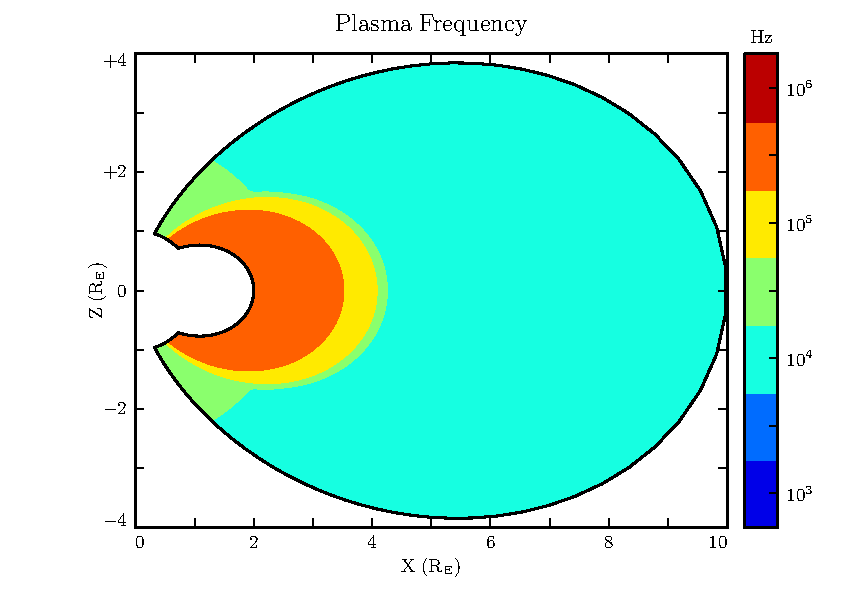
\includegraphics[width=\textwidth]{figures/op.pdf}
    \caption[Plasma Frequency Profile]{
      The plasma frequency reaches a peak value just under \SI{e6}{\Hz} near the equator. Outside the plasmasphere, its value is closer to \SI{e4}{\Hz}, which is still not well-resolved by Tuna's usual time step.  
    }
    \label{fig_op}
\end{figure}

As mentioned in \cref{ch_math} and shown in \cref{fig_op}, plasma oscillation is quite fast -- several orders of magnitude smaller than Tuna's time step as determined in \cref{sec_coords} (\about\SI{10}{\us}). This poses a conundrum. At Tuna's usual time step, the plasma oscillation becomes unstable within seconds\footnote{For stability, $\op \dt < 1$ is necessary. }. On the other hand, reducing the time step by three orders of magnitude to resolve the plasma oscillation is computationally infeasible; a run slated for an hour would require six weeks to complete. 

As it happens, this problem can be solved by artificially increasing the parallel electric constant above its usual value of \ez. Doing so lowers both the speed of light and the plasma frequency within the simulation. 

This technique -- and others like it -- has been widespread in numerical modeling since it was presented by Boris in 1970\cite{boris_1970}. More recently, Lysak and Song considered its use specifically for the case of electron inertial effects\cite{lysak_2001}. The following paraphrases their argument. 

Supposing that the current and electric field are oscillating at frequency $\omega$, the parallel components of \amplaw and \ohmlaw can be written
\begin{align}
  - i \omega \ez E_z &= \oomz \lr{ \, \curl{B} \, }_z - J_z & - \frac{i \omega}{\nu} J_z &= \sz E_z - J_z
\end{align}

Then, eliminating the current, the parallel electric field can be related to the curl of the magnetic field by\footnote{From \cref{def_basics}, $c^2 \equiv \frac{1}{\mz \ez}$ and $\sz \equiv \frac{n e^2}{\me \nu}$ and $\op^2 \equiv \frac{n e^2}{\me \ez}$. }
\begin{align}
  \label{boris_criterion}
  \lr{ 1 - \frac{\omega^2 - i \nu \omega}{\op^2} } E_z &= \frac{c^2}{\op^2} \lr{ \nu - i \omega } \lr{ \, \curl{B} \, }_z
\end{align}

In \cref{boris_criterion}, $\frac{c}{\op}$ is the electron inertial length. While the speed of light and the plasma frequency each depend on \ez, their ratio does not. This allows an estimation of how much the model should be affected by an artificially-large electric constant (and thus an artificially-small plasma frequency): so long as $\frac{\omega^2 - i \nu \omega}{\op^2}$ remains small compared to unity, the model should behave faithfully. 

For waves with periods of a minute or so, even perhaps-implausibly large Boris factors are allowed; for example, increasing \ez by a factor of \num{e6} gives $\left| \frac{\omega^2 + i \omega \nu}{ \op^2 } \right| \lesssim 0.01$. %In some places, this causes the speed of light to fall below the \Alfven speed; R{\"o}nnmark\cite{ronnmark_2000} terms this behavior ``anisotropic vacuum.''

%\todo{Generalized \ohmlaw, in case we decide we need it. Could talk through why all of the other terms are OK to neglect.  
%\begin{align}
%  \vec{E} + \vec{U} \! \times \! \vec{B} & = 
%  \eta \vec{J} + \tfrac{\me}{n e^2} \lrb{
%    \tfrac{\partial}{\partial t} \vec{J} + \nabla \cdot \lr{ 
%      \vec{J} \, \vec{U} + \vec{U} \,\vec{J} +
%      \tfrac{1}{n e} \vec{J} \, \vec{J} } } +
%  \tfrac{1}{n e} \vec{J} \! \times \! \vec{B} -
%  \tfrac{1}{n e} \div{ \vec{P_e} }
%\end{align}
%}

% -----------------------------------------------------------------------------
% -----------------------------------------------------------------------------
% -----------------------------------------------------------------------------
\section{Parallel Currents and Electric Fields}

As discussed in \cref{sec_implications}, parallel electric fields in this regime are expected to be six or more orders of magnitude smaller than the perpendicular electric fields. Numerical results show general agreement: in \cref{fig_electric_field_snapshots}, the parallel electric field appears comparable to its perpendicular counterparts only after its been scaled up by six orders of magnitude. 
\begin{figure}[!htb]
    \centering
    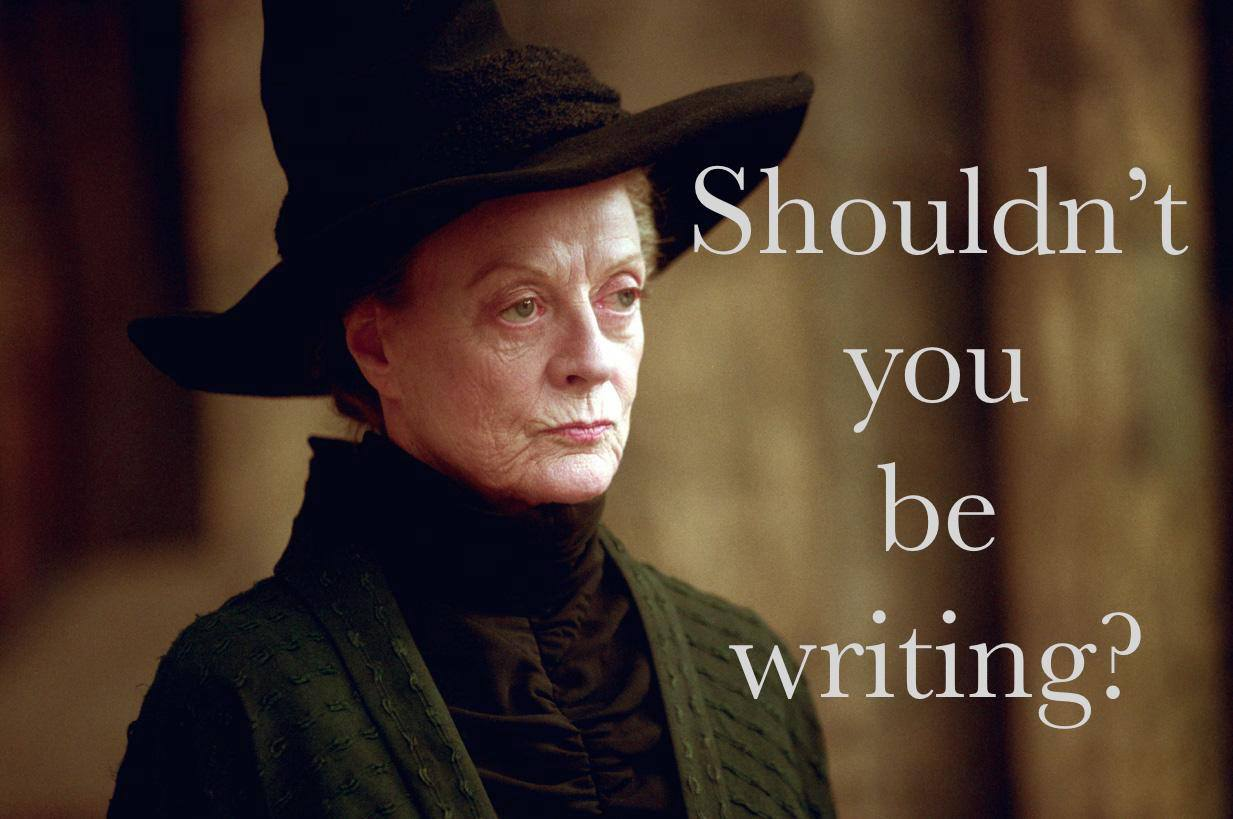
\includegraphics[width=\textwidth]{figures/placeholder.jpg}
    \caption[Electric Field Snapshots]{
      Parallel electric fields are smaller than perpendicular electric fields by about six orders of magnitude. As a result, parallel electric fields do not contribute significantly to $\curl{E}$ in \farlaw. 
    }
    \label{fig_electric_field_snapshots}
\end{figure}

As such, the inclusion of electron inertial effects does not appreciably impact the simulation's gross behavior; in \farlaw, \curl{E} is essentially unaffected. Side by side snapshots of the magnetic fields in runs carried out with and without electron inertial effects are not visibly distinguishable\footnote{In a sense, this is reassuring. It ensures that the present section does not cast doubt on the results presented in \cref{ch_results}, where electron inertial effects are neglected. }

Even if there is no significant feedback through \farlaw, it's informative to consider the structures that arise in parallel currents and electric fields driven by perturbations in the ring current. 

For example, the parallel electric field is at its maximum value in the ionosphere. This makes its structure qualitatively resemble the Poynting flux than the perpendicular electric field components. 

It is furthermore notable that the parallel electric field (and the parallel current that comes from it) exhibits real and imaginary components of comparable magnitude. 

\begin{figure}[!htb]
    \centering
    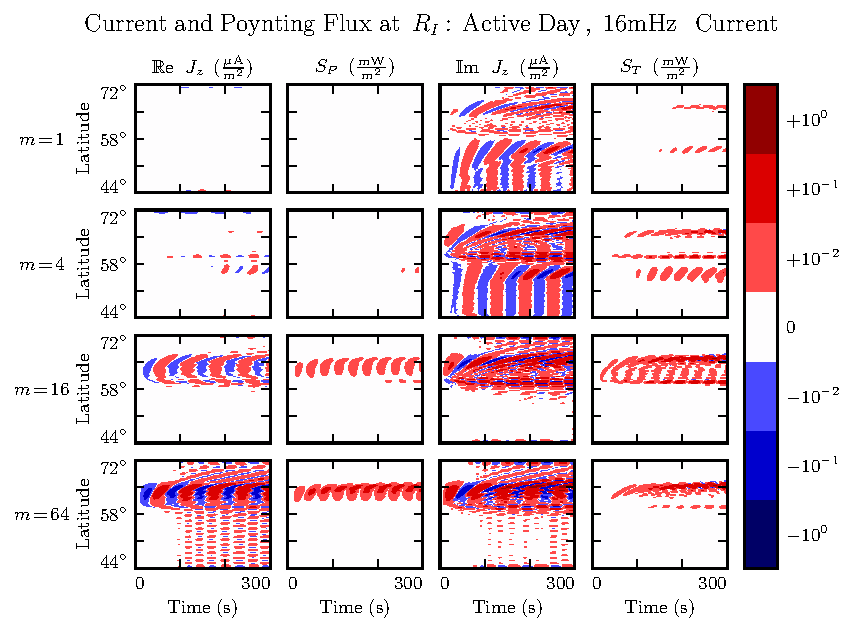
\includegraphics[width=\textwidth]{figures/current_poynting_flux.pdf}
    \caption[Current and Poynting Flux at the Ionosphere]{
      Perhaps unsurprisingly, field-aligned current structures at the ionospheric boundary line up with Poynting flux structures. The imaginary component of the current lines up with the toroidal Poynting flux (which is the product of imaginary $E_x$ and imaginary $B_y^*$), while the real current lines up with the poloidal Poynting flux ($E_y$ and $B_x^*$ are real).
    }
    \label{fig_current_poynting_flux}
\end{figure}

As mentioned in \cref{ch_model}, each field's real component gives its behavior in the meridional plane where the (real) driving is delivered, while imaginary components are representative of waves offset in the azimuthal direction. The Hall conductivity in the ionosphere muddles this relationship somewhat by directly coupling the perpendicular electric field components to one another; even so, the poloidal field components ($B_x$, $E_y$, and $B_z$) are overwhelmingly real while toroidal components ($E_x$ and $B_y$) are overwhelmingly imaginary. 

The parallel electric field and current defy this pattern. The real current scales more or less proportionally with the poloidal Poynting flux, and its imaginary component scales comparably with the toroidal Poynting flux. Rather than being preferrentially coupled to one mode or the other, parallel currents seem to arise wherever energy is moving along the background magnetic field. 

It bears noting further that the Poynting flux waveforms are rectified -- they primarily carry energy Earthward. The current, on the other hand, alternates between upward and downward flow. This effect presumably arises because the current is a linear quantity while the Poynting flux is quadratic: the electric and magnetic fields that make it up oscillate in phase, so their product is positive even when they are negative. 

\begin{figure}[!htb]
    \centering
    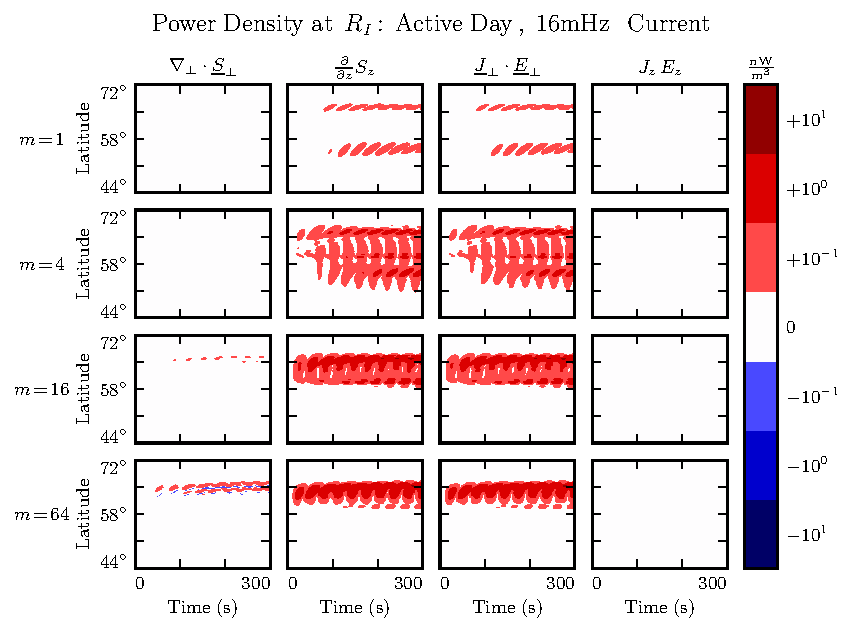
\includegraphics[width=\textwidth]{figures/power_density.pdf}
    \caption[Power Density at the Ionosphere]{
      While field-aligned currents can be of significant size, they are not particularly good at depositing energy in the ionosphere. Energy deposited by the Poynting flux matches closely with Joule dissipation from the perpendicular currents, while $J_z E_z$ is smaller by several orders of magnitude. 
    }
    \label{fig_power_density}
\end{figure}

It's also possible to consider the effect of parallel currents and electric fields on the ionosphere's energy budget, per Poynting's theorem:
\begin{align}
  -\ddt u &= \div{E} + \vec{J} \cdot \vec{E}
\end{align}

As shown in \cref{fig_power_density}, little energy transfer in the ionosphere is mediated by perpendicular components of the Poynting flux. The parallel component of $\vec{J} \cdot \vec{E}$ is comparably unimportant. The energy deposited in the ionosphre by the Poynting flux matches closely with the energy lost to Joule dissipation -- as it should, to conserve energy -- but according to the model, parallel currents and electric fields do not contribute significantly. 

%\todo{Parallel electric fields, supposedly, only appear at high altitude. \cite{marklund_1997,carlson_1998}. }

%\todo{Integrate up a parallel electric field to see the potential difference. Compare to the relation seen by \cite{olsson_1996}, $J_\parallel \sim \Psi_\parallel$ by a proportionality constant of \SIrange{e-8}{e-10}{\S/\meter\squared}. }

% -----------------------------------------------------------------------------
% -----------------------------------------------------------------------------
% -----------------------------------------------------------------------------
\section{Inertial Length Scales}
  \label{sec_lengths}

It's not quite fair to compare the parallel and perpendicular contributions to \curl{E} as was done in the previous section. Perpendicular electric fields are on the order of \SI{1}{\mV/\m}, with wavelengths on the order of \SI{e5}{\km}; they give rise to magnetic field gradients around \SI{0.1}{\nT/\s}. Parallel electric fields, closer to \SI{e-6}{\mV/\m}, would need to vary over length scales of \SI{0.1}{\km} to match with that. 

Such scales are believable. The characteristic length scale of the plasma oscillation is the electron inertial length, $\frac{c}{\op}$, which is on the order of \SI{1}{\km} in the auroral ionosphere and \SI{0.1}{\km} in the low-altitude plasmasphere. However, such lengths are not resolved by Tuna's usual grid; its resolution bottoms out closer to \SI{10}{\km}. 

That is, with the inclusion of electron inertial effects, Tuna's grid is not sufficiently fine to resolve all of the waves expected to be present. The model is prone to instability as a result; see, for example, the ``wigglies'' in the bottom row of \cref{fig_current_poynting_flux} (in the previous section). 

\cref{fig_inertial_length} shows a run with perpendicular resolution smaller than the electron inertial length, side by side with an analogous run on the usual grid. In order to carry out the inertial-scale run, several concessions were made to computational cost. The run simulates only a duration of \SI{100}{\s} (other results in previous sections and in \cref{ch_results} show \SI{300}{\s}), and the grid covers only the auroral latitudes from $L=5$ to $L=7$. 

\begin{figure}[!htb]
    \centering
    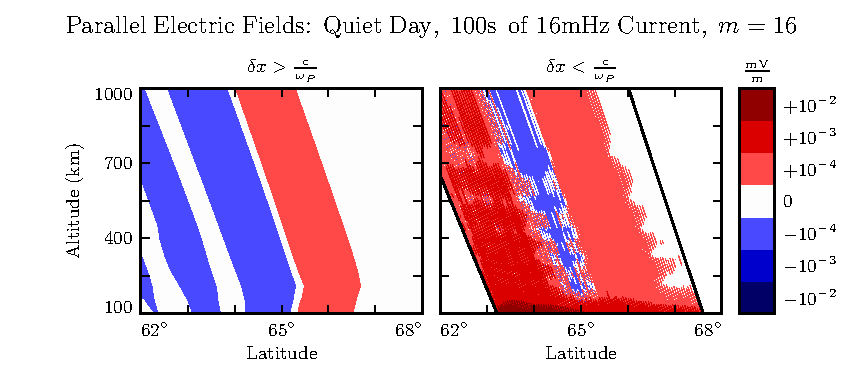
\includegraphics[width=\textwidth]{figures/inertial_length.pdf}
    \caption[Parallel Electric Fields by Perpendicular Grid Resolution]{
      The parallel electric field develops significant structure when the perpendicular grid resolution is smaller than the electron inertial length. Unfortunately, such runs are prohibitively expensive. The lower panel -- which still fails to resolve wave structure properly -- represents a 100-fold increase in computational time. 
    }
    \label{fig_inertial_length}
\end{figure}

Even so, the run presents a significant computational expense. Spread over 16 cores, a \SI{100}{\s} run on Tuna's usual grid takes well under an hour. The inertial-scale run barely finished in 96 hours, the cutoff at the Minnesota Supercomputing Institute\footnote{Runtime goes as the inverse square of grid resolution. Not only does finer resolution require more grid cells, but it also gives rise to proportionally smaller crossing times, imposing a smaller time step. }.

The snapshot shown in \cref{fig_inertial_length} uses a perpendicular grid resolution of \SI{0.7}{\km} at the Earthward edge, which just satisfies the Nyquist rate for the minimum inertial length of \SI{1.7}{\km}. It's still too coarse. There is clearly some small-scale structure developing in the ionosphere, but it's not well resolved. The large number of ``wigglies'' portends an imminent crash. 

Electron inertial effects present a promising first-principles-based approach to investigate parallel currents and electric fields associated with field line resonances. Unfortunately, because of the large differences in scale between Pc4 pulsations and the plasma oscillation, the proper deployment of inertial effects presents a prohibitive computational expense. For this reason, results presented in \cref{ch_results} make use of the core version of Tuna presented in \cref{ch_model}, which does not include the effects of electron inertia. 





% %%%%%%%%%%%%%%%%%%%%%%%%%%%%%%%%%%%%%%%%%%%%%%%%%%%%%%%%%%%%%%%%%%%%%%%%%%%%%
% %%%%%%%%%%%%%%%%%%%%%%%%%%%%%%%%%%%%%%%%%%%%%%%%%%%%%%% Building on Mann 1995
% %%%%%%%%%%%%%%%%%%%%%%%%%%%%%%%%%%%%%%%%%%%%%%%%%%%%%%%%%%%%%%%%%%%%%%%%%%%%%

\chapter{Large Modenumber Effects}
  \label{ch_azm}

This chapter is the real moneymaker. 

The overarching motivation for this work is that Pc4 pulsations vary in interesting ways with respect to azimuthal modenumber, and that prior models have been unable to give a good picture of that behavior. 

% =============================================================================
% =============================================================================
% =============================================================================
\section{Finite Poloidal Lifetimes}
  \label{sec_lifetimes}

Radoski\cite{radoski_1974} looked at \Alfven waves, using a cylindrical coordinate system to imitate an ``unwrapped'' dipole. He argued that poloidal waves should asymptotically rotate to the toroidal mode. 

Mann\cite{mann_1995} performed some wave-in-a-box simulations and found the rotation time to be linear in modenumber: $\tau = \frac{d \lambda}{d \omega_A'}$, where $\lambda = \frac{\azm}{2 \pi r}$ and $\omega_A'$ is the spatial derivative of the \Alfven bounce frequency. Soon afterwards\cite{mann_1997}, he supported his simulations analytically. 

\todo{Crunch out $\frac{d \lambda}{d \omega_A'}$. Preliminary indications are that it doesn't translate well to a realistic grid, but let's double check. }

Ding\cite{ding_1995} ran simulations more-or-less concurrent with Mann's. Ding saw a rotation from poloidal to toroidal... then back again. It seems that the reversal was a spatial resolution issue. 

The aforementioned models made significant simplifying assumptions in terms of geometry and boundary conditions. 

Mann used straight field lines, a uniform \Alfven speed gradient, and perfectly conducting boundaries. 

Ding's simulation is nominally carried out in a dipole geometry, but the ionospheric boundary is at \SI{2.5}{\RE}. Boundaries are also perfectly conducting. 

That is, the results below offer a significantly higher level of realism than any past simulation (in part, of course, because computers are a lot better than they were 20 years ago). 

A dedicated 3D treatment of this problem is unlikely at present. Large azimuthal modenumbers are expensive to compute. That's the whole point! 

%\todo{Do we see a difference between \vec{k} (momentum) and the group velocity? Poynting flux will always be pretty much along the field line, since $B_3$ is small and $E_3$ is zero, but the wave vector need not be. This is a question of coupling/converting to compressional waves, I guess. }

%\todo{Look at McKenzie and Westphal. Waves incident on the bow shock, etc, at weird angles. }

%\todo{Look at the E to B ratio. Compare to the \Alfven speed and to the height-integrated Pedersen conductivity. }

The energy is obtained by integrating (using the Jacobian to handle the grid properly) $U = \int dU = \int u \, dV$. Values are the log (base 10) of that, in the slightly odd units of gigajoules per radian. A factof of 2$\pi$ wouldn't change anything, of course, but it seems inappropriate to integrate all the way around the sphere when Pc4s are longitudinally localized (a fact which was an important part of justifying a 2.5D approach). 

\begin{figure}[H]
    \centering
    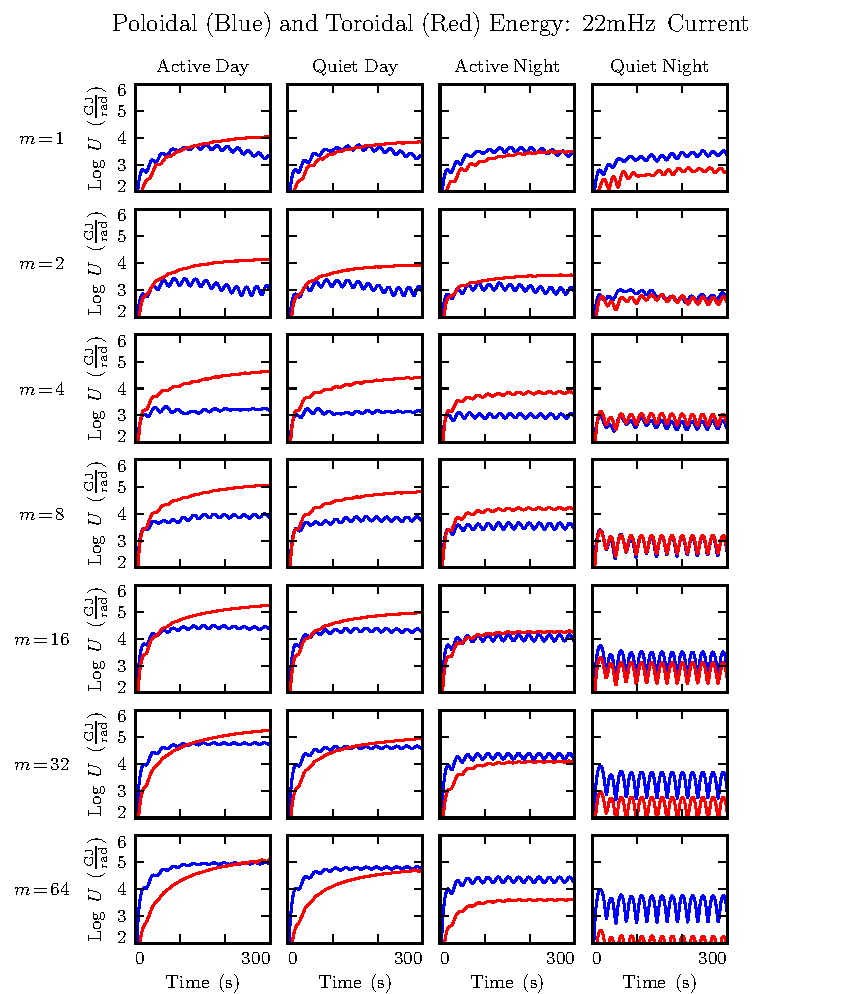
\includegraphics[width=\textwidth]{figures/U_PT_022mHz.pdf}
    \caption[Current-Driven Poloidal and Toroidal Energy: 22mHz]{
      Driving is applied to the poloidal electric field. Over time, the energy rotates from the poloidal mode to the toroidal. The rotation time is affected by the azimuthal modenumber. Ionospheric conductivity also plays an important role. 
    }
    \label{fig_U_PT_022mHz}
\end{figure}

In \cref{fig_U_PT_022mHz}, the rotation of energy from the poloidal mode to the toroidal mode is clear. Driving is strictly poloidal, yet the toroidal mode accumulates energy over time, and doesn't appear to give it back. The rotation happens faster for low-\azm simulations, qualitatively consistent with Mann's result; the time at which poloidal and toroidal energies are equal seems to even be linear in \azm, at he predicted (for well-behaved runs, at least). 

At least, that's the case on the dayside, where the ionosphere is highly conducting. 

On the nightside, the same isn't true in any meaningful way. Dissipation seems to outstrip rotation. Energy does not accumulate over numerous driving periods, as would be expected in resonance; it follows the driving up and down, as a damped-driven oscillator. 

There is evidence that the rotation is still trying to happen. At low \azm, energy is distributed between the poloidal and toroidal mode before dissipating; at high \azm, the energy dissipates straight out of the poloidal mode, never having had a chance to rotate. 

% =============================================================================
% =============================================================================
% =============================================================================
\section{Resonant Shells}
  \label{sec_shells}

Looking a bit deeper, it's possible to comment on the structure of the poloidal and toroidal modes, not just their magnitudes. 

(The following commentary applies to the dayside; on the nightside, there's never much by the way of resonance.)

In \cref{fig_ucolor_pol_022mHz,fig_ucolor_pol_010mHz,fig_ucolor_tor_022mHz,fig_ucolor_tor_010mHz}, electromagnetic energy is binned by field line, averaged over volume (again, with respect to the Jacobian), and plotted as contours. All plots share a color scale. 

The poloidal mode and the toroidal mode exhibit qualitatively different behavior, related to the fact that energy rotates from poloidal to toroidal, and not back. 

At low \azm, energy rotates out of the poloidal mode so quickly that no resonance can form. 

At high \azm, the \Alfven wave is guided. If the driving frequency lines up with the resonant frequency where it's delivered, the poloidal mode resonates strongly. Otherwise, again, no energy accumulates. 

In no case does the poloidal mode demonstrate the ability to move energy across magnetic field lines. 

On the other hand, the toroidal mode does resonate, even if the driving isn't resonant (though in that case the response is of course stronger). The toroidal mode transports energy across field lines until it encounters resonance, then accumulates energy there. Often, resonances are seen in multiple locations due to the non-monotonic \Alfven bounce frequency (recall \cref{fig_fa}) as a function of $L$. 

\begin{figure}[H]
    \centering
    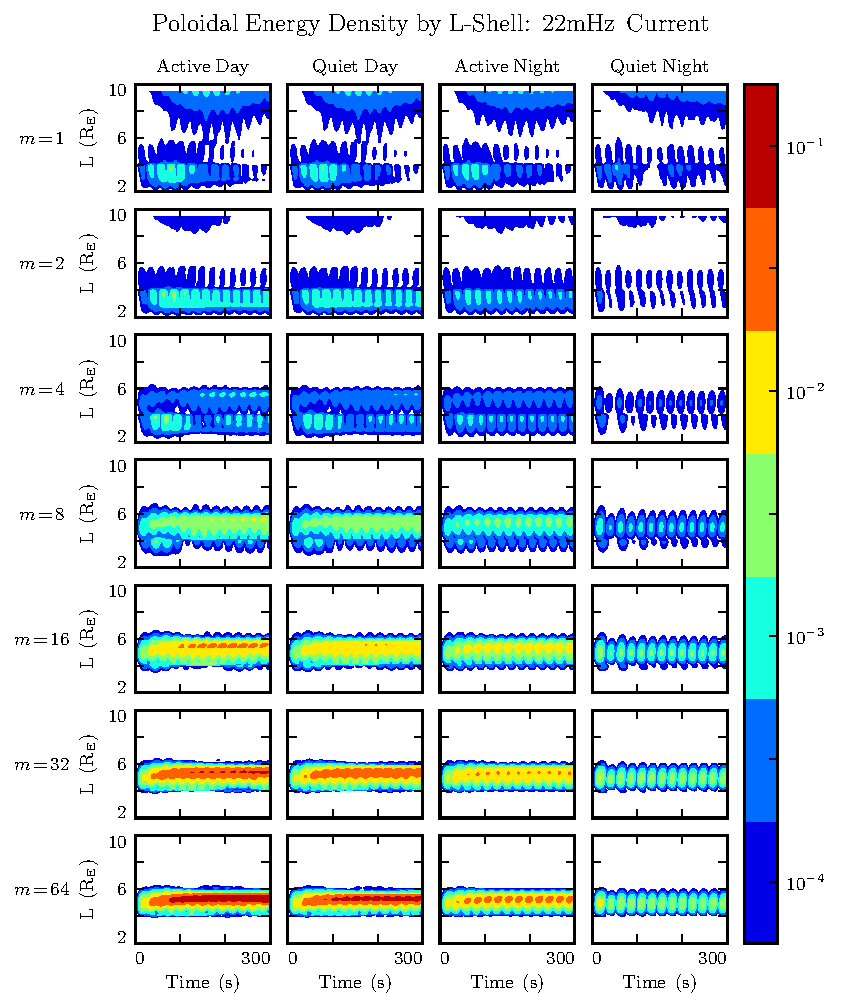
\includegraphics[width=\textwidth]{figures/ucolor_pol_022mHz.pdf}
    \caption[Poloidal Energy Density by L-Shell: 22mHz]{
      If \azm is small, energy rotates to the toroidal mode too fast to form a poloidal resonance. If \azm is large, the \Alfven wave is guided, so it resonates only if the driving frequency lines up with the resonant frequency where it's applied. The result is just one big -- or perhaps even giant -- pulsation. 
    }
    \label{fig_ucolor_pol_022mHz}
\end{figure}

\begin{figure}[H]
    \centering
    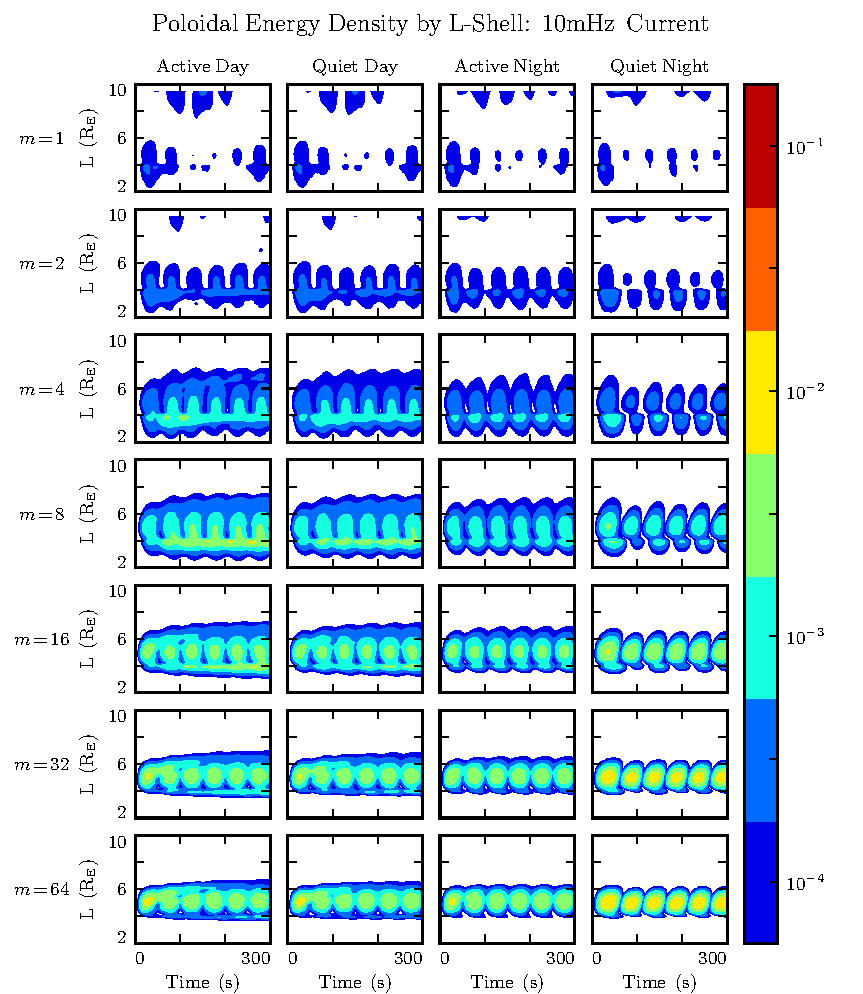
\includegraphics[width=\textwidth]{figures/ucolor_pol_010mHz.pdf}
    \caption[Poloidal Energy Density by L-Shell: 10mHz]{
      When the driving frequency doesn't line up with the location where it's delivered, there's basically no response. There is no movement of energy to a resonant field line, so no energy can accumulate over the course of multiple rounds of driving. 
    }
    \label{fig_ucolor_pol_010mHz}
\end{figure}

\begin{figure}[H]
    \centering
    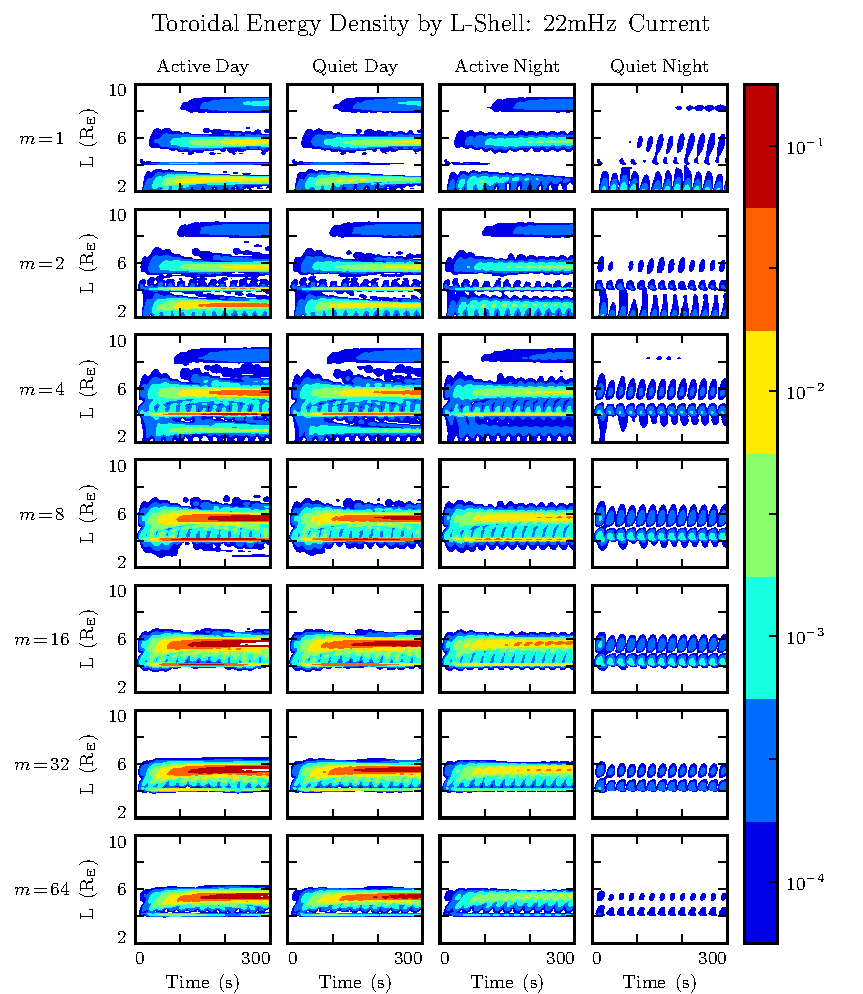
\includegraphics[width=\textwidth]{figures/ucolor_tor_022mHz.pdf}
    \caption[Toroidal Energy Density by L-Shell: 22mHz]{
      If the driving lines up with a nearby field line, the toroidal mode goes crazy! Resonance inside the plasmasphere. Resonance at the plasmapause. Resonance at the driving location. And (weak) attempt at a higher harmonic further out. 
    }
    \label{fig_ucolor_tor_022mHz}
\end{figure}

\begin{figure}[H]
    \centering
    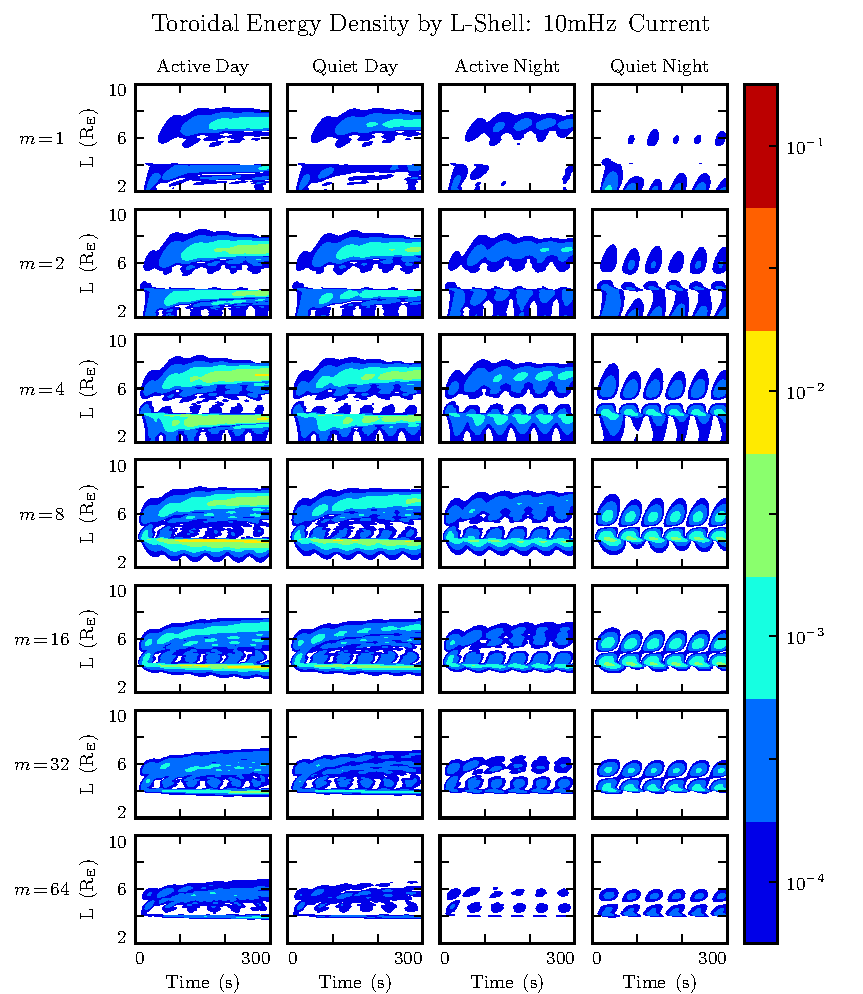
\includegraphics[width=\textwidth]{figures/ucolor_tor_010mHz.pdf}
    \caption[Toroidal Energy Density by L-Shell: 10mHz]{
      Even when not driven resonantly, the toroidal mode still makes the best of its situation. It steals what energy it can from the poloidal mode, carries it to the resonant $L$-shell, and gets to work. (In contrast, recall from \cref{fig_ucolor_pol_010mHz}, in this situation the poloidal mode just does not accumulate energy.)
    }
    \label{fig_ucolor_tor_010mHz}
\end{figure}

% =============================================================================
% =============================================================================
% =============================================================================
\section{Significance for Giant Pulsations}

Giant pulsations are (probably\cite{takahashi_2011}) fundamental mode poloidal Pc4 pulsations with frequencies around \SI{10}{\mHz} and azimuthal modenumbers around \num{20}. They are large, and can sometimes be observed on the ground. 

While this model makes no particular distinction between a giant pulsation and any other Pc4, the above results do line up with giant pulsation observations. 

Giant pulsations aren't seen at small \azm. As shown in \cref{sec_lifetimes}, low-\azm poloidal modes rotate to the toroidal mode too quickly to resonate effectively, even in the case of continuous driving at a locally-resonant frequency. The sweet spot seems to be around $\azm = 20$, more or less the same point where resonance becomes visible in \cref{fig_ucolor_pol_022mHz}. Admittedly, giant pulsations are typically closer to \SI{10}{\mHz} than \SI{22}{\mHz}. It seems likely that qualitatively similar results would be encountered if the driving were moved to an $L$-shell with a bounce time of \SI{10}{\mHz}. 

(Giant pulsations are seen at very large \azm, though not on the ground\cite{takahashi_2013}, due to damping by the ionosphere.)

\todo{Show some ground signatures. They get weak as \azm gets large. }

Giant pulsations are monochromatic, and can be accompanied by ``multiharmonic toroidal waves''\cite{takahashi_2011}. Per \cref{sec_shells}, this is about what would be expected from a mishmash of poloidal driving. Poloidal modes of all frequencies rotate into the toroidal mode; resonant poloidal modes resonate; non-resonant poloidal modes become evanescent. 

Giant pulsations often drift azimuthally. This model can't resolve azimuthal drift directly, of course, but can fake it by looking at complex phase. There has been some indication (not shown) of complex phase rotation in ground magnetic fields. However, at the boundary, it's difficult to disentangle which values are imaginary to indicate an azimuthal offset, and which are imaginary because of Hall coupling. Investigation is ongoing. 

% =============================================================================
% =============================================================================
% =============================================================================
\section{Electromagnetic Energy Gap}

\todo{A preliminary search (and asking Bob) has not turned up anyone looking at this before, so it's hard to provide context. }

Above, we considered the decay of energy from the poloidal mode to the toroidal mode. A natural follow up is, are there any other surprising trends in the distribution of energy?

As it turns out, yes!

In cases where the driving frequency does not line up with the local bounce frequency, energy doesn't accumulate particularly well in either the poloidal or the toroidal mode. Like a damped-driven oscillator, the system's behavior follows the input. 

At low \azm, what energy there is divides itself more-or-less equally between the electric and magnetic fields. 

As \azm increases, oddly, a gap appears. When the conductivity is high, the magnetic field holds more energy than the electric field. The disparity can be up to a factor of $\sim \num{3}$; that is, \SI{75}{\percent}. of the energy in the magnetic field, and \SI{25}{\percent} in the electric field. When conductivity is low, the opposite happens: energy concentrates in the electric field. 

This lines up somewhat with what might be expected. When conductivity is low, it takes a larger electric field to induce the same current, and thus the same magnetic field. But it's not clear why this disparity only appears at large \azm, or why it does not appear when the driving is resonant. 

Maybe it's a timing issue? A relationship between the bounce time (which is more or less indepedent of \azm) and the rotation time (which depends on \azm). 

\todo{How is the compressional magnetic field brought into these calculations? It exists only at small \azm. It's never particularly large, it also gets added to the zeroth-order field before squaring. }

\begin{figure}[H]
    \centering
    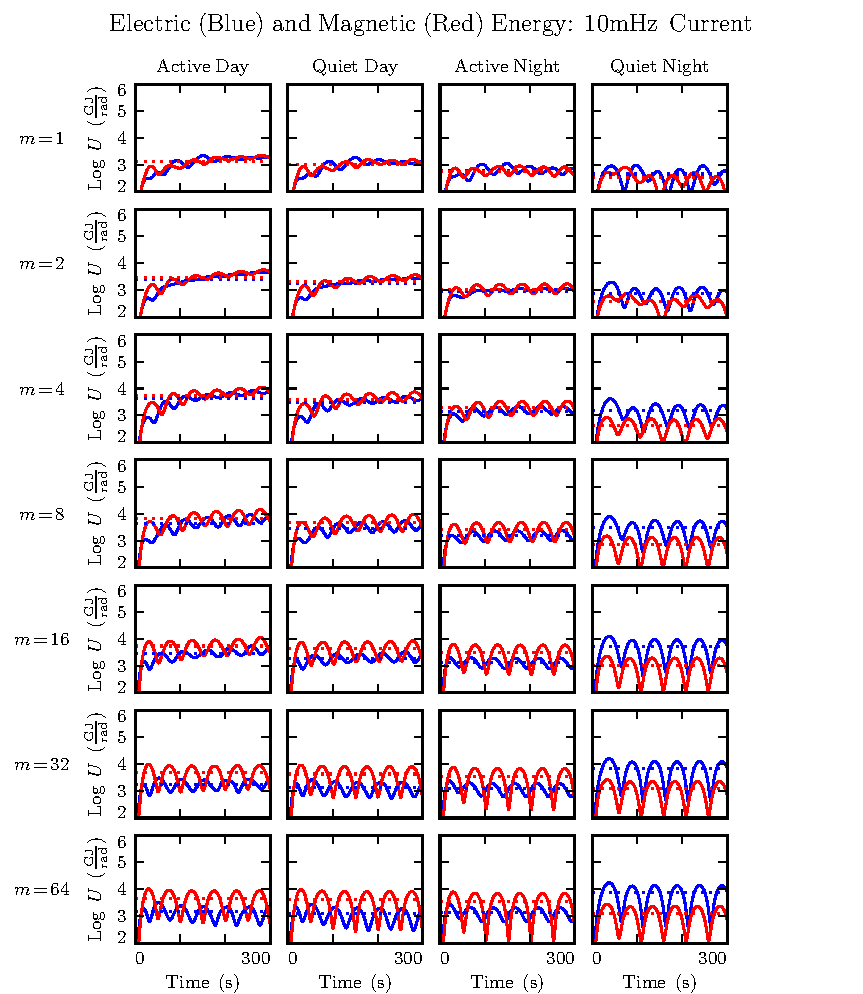
\includegraphics[width=\textwidth]{figures/U_BE_010mHz.pdf}
    \caption[Current-Driven Electric and Magnetic Energy: 10mHz]{
      In the absence of resonant driving, a disparity emerges at large \azm between the energy in the magnetic field and the energy in the electric field. The sign of the difference depends on the ionospheric conductivity. 
    }
    \label{fig_U_BE_010mHz}
\end{figure}


\begin{figure}[H]
    \centering
    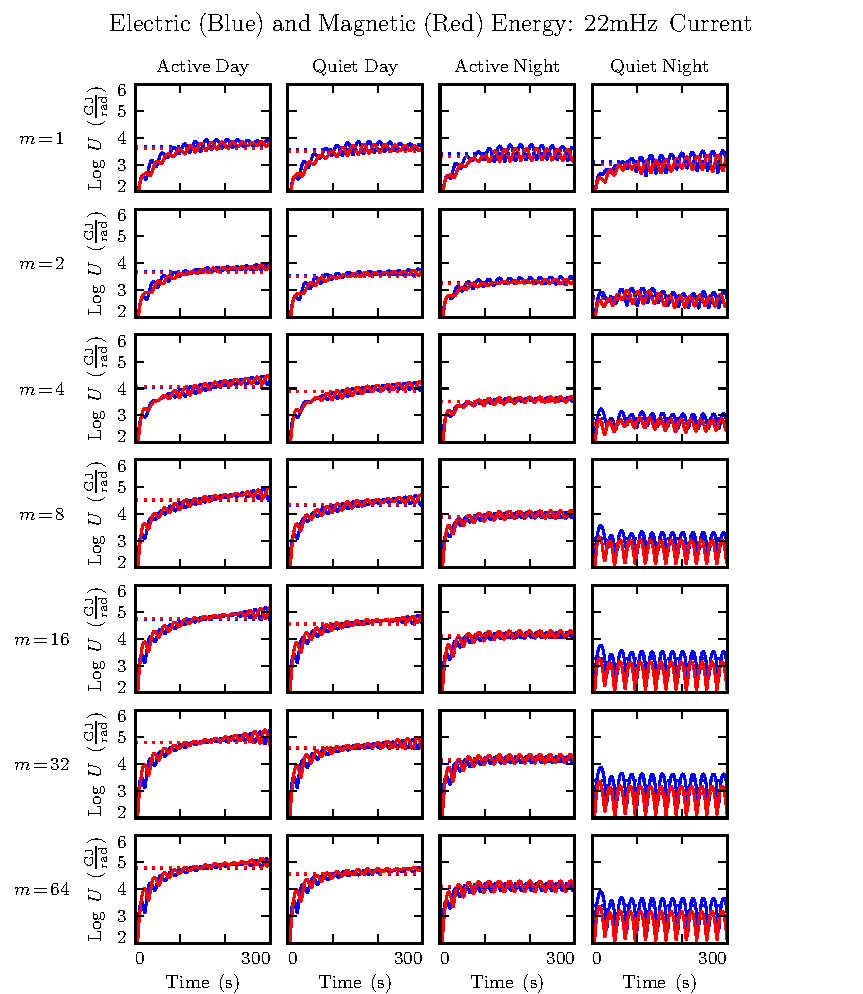
\includegraphics[width=\textwidth]{figures/U_BE_022mHz.pdf}
    \caption[Current-Driven Electric and Magnetic Energy: 22mHz]{
      When driving is resonant, energy is distributed almost exactly half-and-half between the electric and magnetic fields, regardless of \azm. The rightmost profile still shows a gap, likely because the ionospheric conductivity in that model is low enough that nothing ever resonates. 
    }
    \label{fig_U_BE_022mHz}
\end{figure}


















\chapter{Van Allen Probe Observations}
  \label{ch_rbsp}

The results presented in \cref{ch_results} are interesting on their own, but become particularly valuable when combined with observational data. Unfortunately, only a small number of studies to date have explored how Pc4 observation rate is affected by the harmonic and polarization structure of those waves. 

While Pc4 pulsations have previously been studied in terms of both harmonic\cite{arthur_1981,cummings_1969,engebretson_1988,hughes_1978,singer_1982,takahashi_1984} and polarization\cite{anderson_1990,dai_2015,dai_2013,kokubun_1989,liu_2009}, little work has considered both at the same time. This has largely been due to observational constraints. The classification of a wave's harmonic is best carried out by computing the phase offset of the magnetic and electric field waveforms, simultaneous in situ measurements of which have only recently become available as part of the THEMIS\cite{angelopoulos_2008} and Van Allen Probe\cite{stratton_2012} missions. The Van Allen Probes (launched in 2012) are particularly well-suited to the study of Pc4 pulsations as their apogee of $L \sim 6$ coincides closely with eigenfrequencies in the Pc4 range. 

The present chapter uses data from the Van Allen Probes' EFW instrument\cite{wygant_2013} to survey the occurrence rate of FLRs in the Pc4 range as a function of harmonic parity and polarization, as well as magnitude, frequency, and phase. The tools used to perform the present analysis --- SPEDAS and the SPICE kernel --- are publicly available. They, along with the Python routines used to download, filter, and plot the data, can be found in a Git repository at \url{https://github.com/chizarlicious/RBSP}. 

\todo{Set this up, along with Tuna, at \url{https://github.com/chizarlicious/UMN_Space-Physics}. }

%Observations show that the poloidal mode is most excited in the second harmonic\cite{cummings_1969,hughes_1978,arthur_1981,singer_1982,takahashi_1984,engebretson_1988} even when there is a strong compressional component\cite{takahashi_1987,haerendel_1999,vaivads_2001,sibeck_2012}. 

%\todo{The tools used in the present chapter --- SPEDAS and the SPICE kernel --- are publicly available. They run best with an IDL license, which is not, but they are functional using just the (free) IDL virtual machine. The code is wrapped up in a Git repository: \url{https://github.com/chizarlicious/RBSP} (maybe should make a GitHub organization to hold this code, to decouple it from my personal account?). }

% -----------------------------------------------------------------------------
% -----------------------------------------------------------------------------
% -----------------------------------------------------------------------------
\section{Sampling Bias and Event Selection}
  \label{sec_selection}

The present analysis makes use of Van Allen Probe data from October 2012 to August 2015 --- the entire range available at the time of writing. Between the two probes, that's just over 2000 days of observation. 

For the purposes of Pc4 pulsations, it's reasonable to consider the two probes to be independent observers. Nearly all Pc4 events occur near apogee ($L\gtrsim5$), at which point the two probes are several hours apart in MLT. Pc4 events are typically not large enough to be seen by both probes simultaneously, and not long enough in duration to be seen by two probes passing through the same region of space several hours apart. 

\todo{Quantify how often an event is seen by both probes? }

Electric and magnetic field waveforms are collected using the probes' EFW and EMFISIS instruments respectively. Values are cleaned up by averaging over the ten-second spin period. Three-dimensional electric field data is then obtained using the $\vec{E} \cdot \vec{B} = 0$ assumption. Notably, this assumption is taken only when the probe's spin plane is offset from the magnetic field by at least \SI{15}{\degree}. The rest of the data --- about half --- is discarded, which introduces a sampling bias against the flanks. 

A further bias is introduced by the probes' non-integer number of precessions around Earth. As of July 2014, apogee had precessed once around Earth\cite{dai_2015}. The present work considers roughly one and a half precessions; the nightside has been sampled at apogee twice as often as the dayside. 

The spatial distribution of usable data --- that is, data for which three-dimensional electric and magnetic fields are available --- is shown in \cref{fig_pos_all_sharp}. Bins are unitary in $L$ and in MLT. Distribution in magnetic latitude is not shown; the Van Allen Probes are localized to within \about\SI{10}{\degree} of the equatorial plane. 

\begin{figure}[!htb]
    \centering
    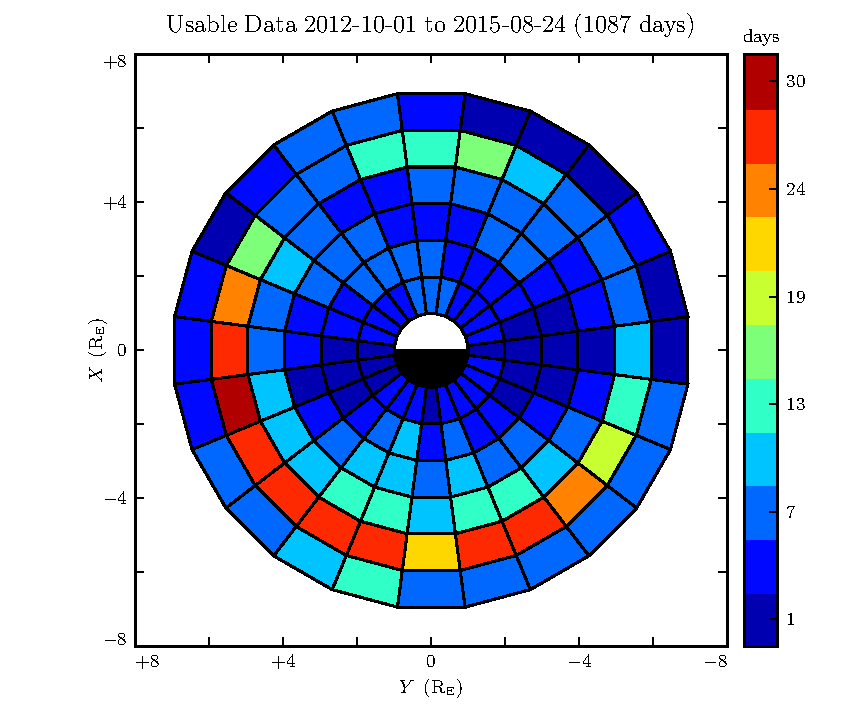
\includegraphics[width=\textwidth]{figures/pos_all_sharp.pdf}
    \caption[Distribution of Usable Van Allen Probe Data]{
      Three-dimensional electric field values are computed by assuming $\vec{E} \cdot \vec{B} = 0$. Data is discarded whenever the magnetic field falls within \SI{15}{\degree} of the spin plane, which introduces a bias against the flanks. Furthermore, the probes have completed one and a half precessions around Earth; the dayside has been sampled once at apogee, and the nightside twice. 
    }
    \label{fig_pos_all_sharp}
\end{figure}

Field measurements are transformed from GSE coordinates into the same dipole coordinates used in \cref{ch_model,ch_results}. The \z axis (parallel to the background magnetic field) is estimated using a ten-minute running average of the magnetic field measurements. The \y axis is set parallel to $\zhat \times \vec{r}$, where \vec{r} is the probe's geocentric position vector. The \x axis is then defined per $\xhat \equiv \yhat \times \zhat$. This scheme guarantees that the axes are right-handed and pairwise orthogonal\cite{liu_2009}. 

The \about1000 days of usable data are considered half an hour at a time, which gives a frequency resolution of \about\SI{0.5}{\mHz} in the discrete Fourier transform. Spectra are computed for all six field components: \dft{B_x}, \dft{B_y}, \dft{B_z}, \dft{E_x}, \dft{E_y}, and \dft{E_z}. The background magnetic field is subtracted before transforming the magnetic field components, leaving only the perturbation along each axis\footnote{As in \cref{ch_model,ch_results}, $B_x$, refers not to the full magnetic field in the \x direction, but to the perturbation in the \x direction from the zeroth-order magnetic field. The same is true for $B_y$ and $B_z$. }. Each waveform is also shifted vertically so that its mean over the thirty minute event is zero. 

Frequency-domain Poynting flux is computed from the electric and magnetic field transforms. A factor of $L^3$ compensates the compression of the flux tube, so that the resulting values are effective at the ionosphere. Poloidal and toroidal Poynting flux, respectively, are given by:
\begin{align}
  \dft{S_P} &\equiv -\frac{L^3}{\mz} \dft{E_y} \dft{B_x^*} &
  \dft{S_T} &\equiv  \frac{L^3}{\mz} \dft{E_x} \dft{B_y^*}
\end{align}

The poloidal and toroidal channels are independently checked for Pc4 waves. For each channel, a Gaussian profile is fit to the magnitude of the Poynting flux, $|\dft{S}\arg{\omega}|$. If the fit fails to converge, or if the peak of the Gaussian does not fall within \SI{5}{\mHz} of the peak value of \dft{S}, the event is discarded. Events are also discarded if their frequencies fall outside the Pc4 frequency range (\SIrange{7}{25}{\mHz}) or if their amplitudes fall below \SI{e-2}{\mW/\m\squared} (out of consideration for instrument sensitivity). 

Events are discarded if their parity is ambiguous. The electric field and the magnetic field must be coherent at a level of 0.9 or better (judged at the discrete Fourier transform point closest to the peak of the Gaussian fit). Any event within \SI{3}{\degree} of the magnetic equator is also not used; as discussed in \cref{ch_flrs}, in order to distinguish an odd mode from an even mode, it's necessary to know whether the observation is made north or south of the equator. 

\todo{How much time do the probes spend within \SI{3}{\degree} of the magnetic equator? }

A visual inspection of events shows that those with broad ``peaks'' in their spectra are typically not peaked at all --- they are noisy spectra with several spectral features grouped just closely enough to trick the fitting routine. A threshold is set at a FWHM of \SI{3}{\mHz} (equally, a standard deviation of \SI{1.27}{\mHz}). Any event with a Gaussian fit broader than that is discarded. 

Notably, events are not filtered on their phase --- that is, on the division of their energy between standing and traveling waves. This is the topic of \cref{sec_phase}. 

\todo{Are we biased in terms of \DST? What's the distribution look like for the good data and for the bad data? }

% -----------------------------------------------------------------------------
% -----------------------------------------------------------------------------
% -----------------------------------------------------------------------------
\section{Events by Mode}
  \label{sec_rate}

The filters described in \cref{sec_selection} yield 762 Pc4 events, the spatial distribution of which is shown in \cref{fig_rate_all_sharp}. In each bin, the event count is normalized to the amount of usable data, per \cref{fig_pos_all_sharp}. Bins shown in white contain zero events. The rate in the bottom corner is an overall mean, weighing each bin equally. 

\begin{figure}[!htb]
    \centering
    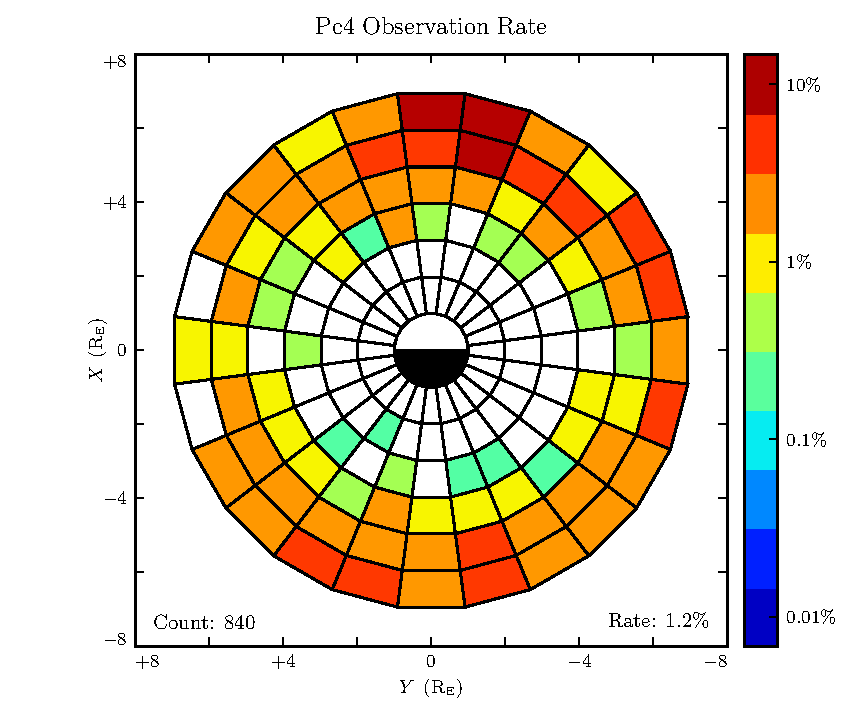
\includegraphics[width=\textwidth]{figures/rate_all_sharp.pdf}
    \caption[Rate of Pc4 Events]{
      The above figure shows the spatial distribution of all 762 observed Pc4 events. Counts are normalized by the amount of usable data in each bin. The value in the bottom-right corner is the mean of the rate in each bin; it's an estimate of how often Pc4 events would be observed if the sampling were distributed uniformly in space. Events where the poloidal and toroidal channel trigger simultaneously (\about\SI{10}{\percent} of cases) are counted as only a single event. Bins shown in white contain zero events. 
    }
    \label{fig_rate_all_sharp}
\end{figure}

Consistent with previous work, Pc4 events peak on the dayside and are rarely observed at $L < 4$. Nearly \SI{30}{\percent} of the usable data shown in \cref{fig_pos_all_sharp} is taken at $L < 4$, yet only 16 of the 762 events appear there. 

On the other hand, the present work runs contrary to Dai's 2015 result in terms of Pc4 event rates with respect to the plasmapause (not shown). His analysis found (poloidal) Pc4 pulsations to be comparably common inside and outside the plasmapause\cite{dai_2015}. In the present work, only 40 of the 762 events (\SI{5}{\percent}) fall inside the plasmasphere, despite the fact that \SI{40}{\percent} of the available data falls within the plasmasphere. The disparity is not likely due to a difference in sampling --- Dai's work, like the present work, uses data from the Van Allen Probes mission. Rather, the difference is likely due to disagreement in how the plasmapause is defined. Dai identifies the plasmapause by the maximum gradient in electron number density, while the present work takes an electron density of \SI{100}{\percc} to mark the plasmapause\footnote{Per ongoing work by Thaller. }. 

The same events in \cref{fig_pos_all_sharp} are shown again in \cref{fig_mode_all_sharp}, partitioned by polarization and parity. 

\begin{figure}[!htb]
    \centering
    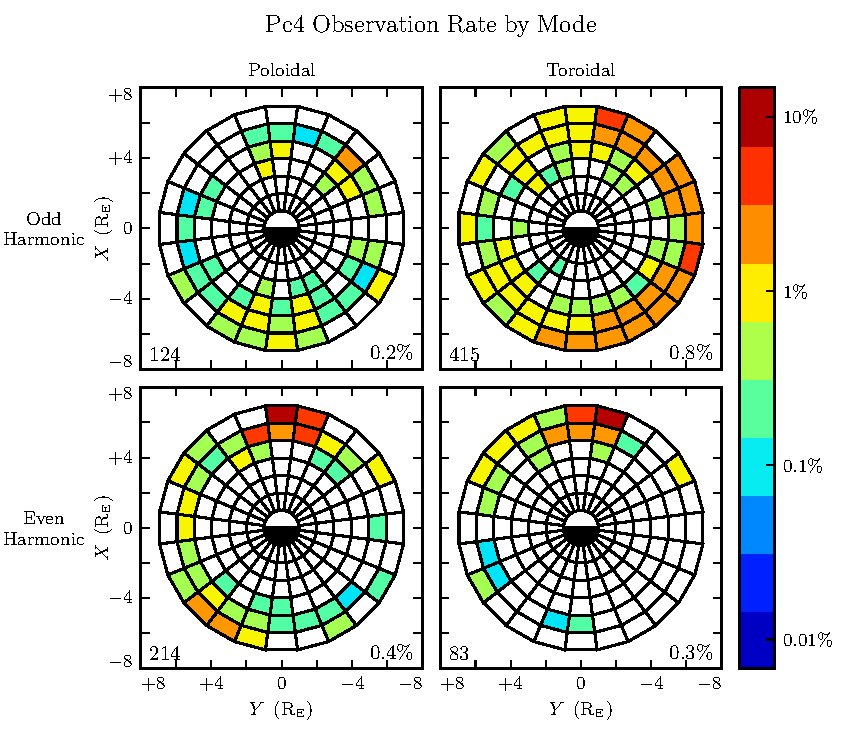
\includegraphics[width=\textwidth]{figures/mode_all_sharp.pdf}
    \caption[Rate of Pc4 Events by Mode]{
      The above figure shows the spatial distribution for the same 762 events shown in \cref{fig_rate_all_sharp}, partitioned by polarization and parity. The selection criteria described in \cref{sec_selection} ensure that both properties are known for all events. Event counts are normalized by the time spent by the amount of usable data in each bin. Counts shown in the bottom-left corners do not sum to 762 because some events trigger on both the poloidal channel and the toroidal channel. Bins shown in white contain zero events. 
    }
    \label{fig_mode_all_sharp}
\end{figure}

The distribution of even poloidal events in \cref{fig_mode_all_sharp} is consistent with that reported by Dai\cite{dai_2015}: the observation rate is peaked at noon, and smeared across the dusk side. Notably, Dai's work focused on even poloidal waves. While he did not explicitly remove odd events from his sample, he did introduce a threshold in the magnetic field. This threshold is preferrentially satisfied by even waves (which have a magnetic field antinode near the equator) compared to odd waves (which have a magnetic field node). Dai characterized the parity of only a quarter of his events; among those, he found even harmonics to outnumber odd harmonics ten-to-one. 

In fact --- to the degree that they can be straightforwardly compared --- the distributions in \cref{fig_mode_all_sharp} also show agreement with work by Anderson\cite{anderson_1990} (using AMPTE/CCE), Kokubun\cite{kokubun_1989} (using ATS6), Liu\cite{liu_2009} (using THEMIS), and Motoba\cite{motoba_2015} (using GOES). Toroidal events dominate overall, and are primarily seen on the morning side. Poloidal events are spread broadly in MLT, with a peak near noon and distinctive odd harmonics in the early morning. 

Crucially, the present work can offer insight into how previous results fit together. Unlike events considered in previous works, those shown in \cref{fig_mode_all_sharp} have all been categorized in terms of both polarization and parity. And, perhaps more importantly, the selection process has not introduced a bias with respect to polarization or parity (at least not an obvious one). 

The even events shown in \cref{fig_mode_all_sharp} show good agreement with the numerical results in \cref{ch_results}. The distributions are qualitatively similar, as might be expected if even poloidal waves served as a source for even toroidal waves. Even poloidal waves are more prevalent, suggesting a typical event duration comparable to the poloidal-to-toroidal rotation timescale. And even toroidal events are skewed dayward compared to even poloidal events, suggesting that poloidal-to-toroidal rotation is inhibited by increased Joule dissipation on the nightside. 

The same can be said to some extent for the odd events in \cref{fig_mode_all_sharp}, though the trends are less strong. Odd poloidal and odd toroidal events are both scarce on the dusk flank. On the dawn flank, poloidal events skew nightward, while toroidal events are spread broadly --- that is, they are skewed dayward compared to the poloidal events. However, it's unclear why odd toroidal events outnumber odd poloidal events to such a degree. 





Not only does \cref{fig_mode_all_sharp} show that toroidal events outnumber poloidal events, but it also shows that toroidal events are predominantly odd harmonics --- as opposed to the primarily-even poloidal events. 








This may suggest that odd poloidal waves are more likely than even ones to be driven at low modenumber (allowing a prompt rotation of that energy to the toroidal mode). One might expect low-\azm poloidal modes to be driven by a broad, sudden change in solar wind dynamic pressure, for instance. The relative scarcity of odd poloidal observations on the dayside may indicate a short-lived source. At low \azm, energy rotates to the toroidal mode on the order of a wave period; without an ongoing source, there would be no poloidal wave to observe. 





\todo{Actually, it looks like odd poloidal waves are split about half-and-half around $\left| \frac{B_z}{B_x} \right| = 0.2$. Compressional odd modes are more common near midnight. Noncompressional ones are mostly in the morning. Even poloidal events are skewed toward low \azm. This is probably worth showing. }

\todo{Odd poloidal events are skewed nightward compared to odd toroidal events. This is not surprising. Per \cref{ch_results}, nightside poloidal events are less likely to give rise to toroidal events than those on the dayside. Even events too, actually. The toroidal distribution looks like the poloidal distribution, but skewed dayward. }

This would furthermore be consistent with even modes' apparent dearth of ground signatures\cite{takahashi_1992}. If even harmonics tend to be produced at higher modenumber than odd ones, even harmonics would be expected to produce ground signatures less often\footnote{See \cref{attenuation}. }. 

Even poloidal modes and even toroidal modes exhibit similar distributions in space: both are peaked at noon and smeared across the dusk flank, with little activity on the dawn side. This is further support for the even poloidal wave as a significant source for the even toroidal mode. 

\todo{People have talked about this. Is there a conventional explanation for dawn-dusk asymmetry? }

\todo{What else do we want to say here? Or does the rest of the commentary belong in the later sections? Note that plots in future sections are lower resolution, to make sure that the number of bins remains much smaller than the number of events. }

\todo{How does this relate to the numerical results in \cref{ch_results}? }











In \cref{fig_mode_all_sharp}, events are partitioned by parity and polarization, yielding 124 odd poloidal events, 214 even poloidal events, 415 odd toroidal events, and 83 even toroidal events --- a total of 836 events. The total is greater than 762 because in \about\SI{10}{\percent} of events, the poloidal and toroidal channels trigger independently. Such cases are marked as a single event in \cref{fig_rate_all_sharp}, but the toroidal and poloidal events are both shown in \cref{fig_mode_all_sharp}. 














Double-triggering can be taken as a vague proxy for event quality. When the channels both trigger independently, the two events almost always (71 of 74 events) exhibit the same parity. This suggests a poloidal wave with suffient power, and a sufficient narrow spectral peak, that it can still be seen after much of its energy has rotated to the toroidal mode. 

\begin{figure}[!htb]
    \centering
    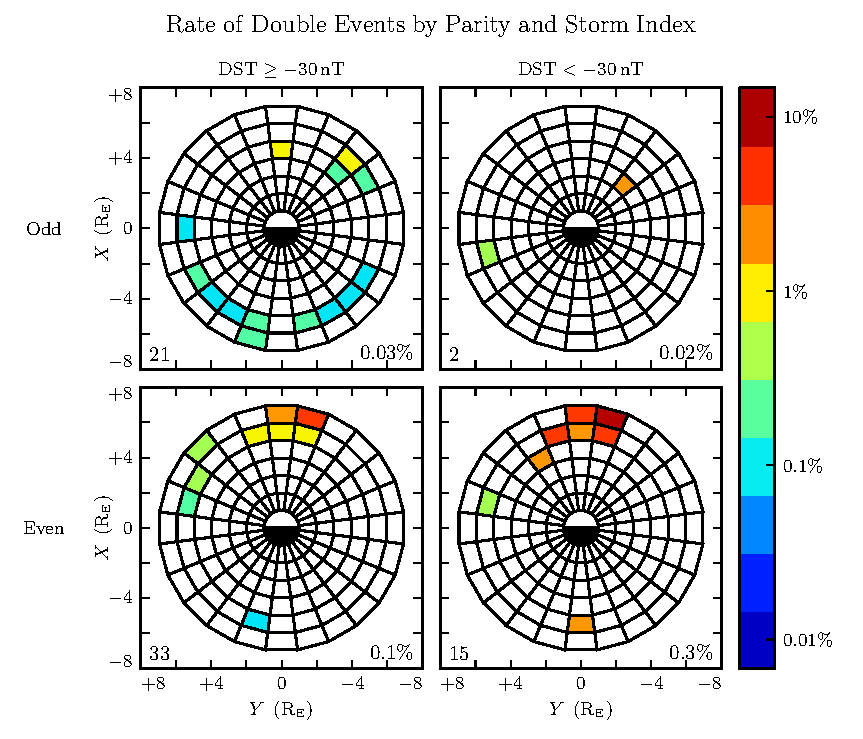
\includegraphics[width=\textwidth]{figures/double_rate_sharp.pdf}
    \caption[Rate of Double Pc4 Events by Parity and Storm Index]{
      A double event is a simultaneous triggering of the poloidal and toroidal channels on the same probe. In such cases, the two channels almost always exhibit the same parity. Double events serve as a vague proxy for event quality --- a poloidal event with sufficient strength and clarity to be seen even after much of its energy has rotated to the toroidal mode. Odd double events are spread broadly; even events are concentrated near noon, and become more common during geomagnetically active times. 
    }
    \label{fig_double_rate_sharp}
\end{figure}

The spatial distribution of double events is shown in \cref{fig_double_rate_sharp}. The left column shows events observed with $\DST \geq \SI{-30}{\nT}$, normalized by the amount of usable data at $\DST \geq \SI{-30}{\nT}$. The right column shows events at $\DST < \SI{-30}{\nT}$, normalized by the amount of data with $\DST < \SI{-30}{\nT}$. 

Odd double-triggering events are spread broadly in MLT. They rarely occur twice on the same day; the 23 events shown take place over 20 different dates. Odd double events occur at similar rates regardless of \DST. 

Even-harmonic double-triggering events, on the other hand, are mostly seen near noon, and are significantly more common during geomagnetically active times. Even events are also more concentrated than odd ones. The 48 even-harmonic double-events shown in the bottom row of \cref{fig_double_rate_sharp} are spread over 20 days, and 35 of them are spread over just 7 days. This clustering --- where the poloidal and toroidal channel both trigger for five to ten half-hour events in the same day --- is prevalent regardless of \DST. 





%Dai\cite{dai_2015} used RBSP to look at poloidal Pc4 events, with a bias in favor of the second harmonic --- 890 events. Events are most common near noon, but are spread across the day and dusk side, with a few stragglers at midnight. 

%Anderson\cite{anderson_1990} used AMPTE/CCE (mostly $L>7$, near the equator) to look at Pc4 events --- 7000 hours. Limited commentary on parity. Toroidal modes were found to outnumber poloidal modes three-to-one. ``Harmonic toroidal resonances'' are spread 0600 to 1600. ``Fundamental toroidal resonances'' (which are not mutually exclusive with harmonic ones!) appear everywhere but dusk. 

%Liu\cite{liu_2009} used THEMIS (equatorial orbit, $L$ out to \about10) to look at both poloidal and toroidal modes --- 9805 one-minute Pc4 events (?). No commentary on parity. Poloidal events are most common at noon (with another peak post-midnight) and strongest on the dusk side. Toroidal events are most common from pre-dawn to pre-noon and strongest pre-midnight and post-dawn. 

%Kokubun\cite{kokubun_1989} used ATS6 (synchronous orbit) --- \about150 events. No commentary on harmonic. Toroidal events dominate in the dawn sector. Poloidal events are spread across all MLT, with a peak in the early afternoon and Pgs in the early morning. 

%Motoba\cite{motoba_2015} used GOES13 and GOES15 (geosynchronous) to look specifically at Pgs --- 105 events. Seen from midnight to noon, with a strong peak before dawn, 0300 or so. 

%\todo{Even poloidal events and even toroidal events are distributed similarly, which is good to see, since even poloidal events give rise to even toroidal events. The relationship is less clear for odd events, though odd poloidal modes and odd toroidal modes are both least common at dusk. }

%\todo{Odd toroidal events are by far the most commonly observed. Oddly, even poloidal events are the least common. }

%\todo{Even modes are less likely to be observed on the ground? \cite{takahashi_1992} }

% -----------------------------------------------------------------------------
% -----------------------------------------------------------------------------
% -----------------------------------------------------------------------------
\section{Events by Amplitude}
  \label{sec_amp}

One might reasonable be concerned that the spatial distributions presented in \cref{fig_mode_all_sharp} are dominated by these small events, while Pc4 events large enough to be noteworthy follow a different distribution entirely. The goal of the present section is to address that concern. 

\begin{figure}[!htb]
    \centering
    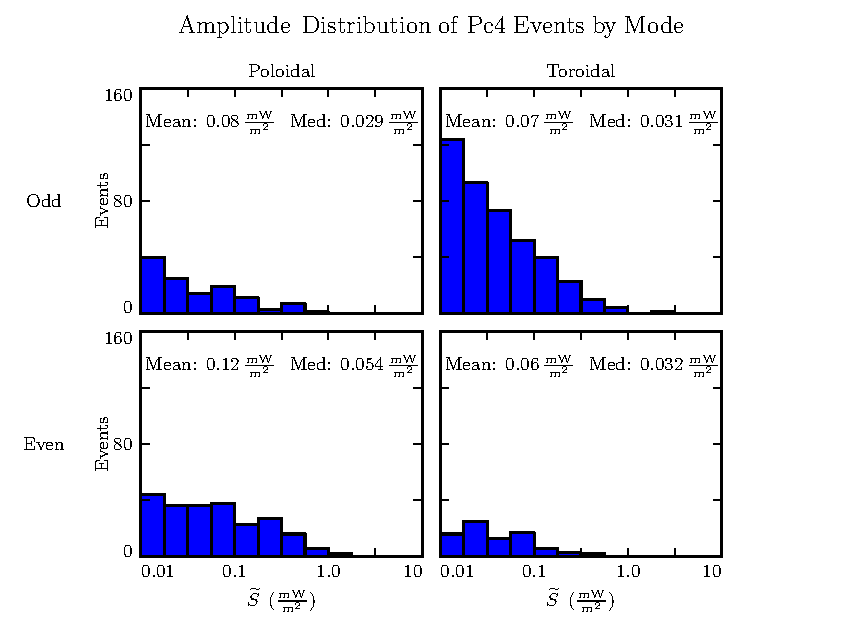
\includegraphics[width=\textwidth]{figures/amp.pdf}
    \caption[Amplitude Distribution of Pc4 Events by Mode]{
      Amplitude distribution is shown for Pc4 events by parity and polarization, based on the peak of the spectrum's Gaussian fit. Odd poloidal events, odd toroidal events, and even toroidal events fall off sharply with increasing amplitude, while the even poloidal events are distributed more broadly --- the mean and median of the even poloidal distribution is twice as large as that of the others. 
    }
    \label{fig_amp}
\end{figure}

The distribution of event magnitudes is presented in \cref{fig_amp}, graded based on the peak of the Gaussian fit of each event's Poynting flux, $|\dft{S}\arg{\omega}|$. Mean and median values are listed for each mode. Most events are small, with Poynting flux well below \SI{0.1}{\mW/\m\squared} when mapped to the ionosphere. Only a handful of events --- 3 out of 762 --- exceed \SI{1}{\mW/\m\squared}, typically taken to be the threshold at which visible auroral arcs form. One such event is shown in \cref{fig_sample_event_strong}. 

\todo{Say something about this event? Not really clear what purpose is served by this example, actually. As a matter of curiosity, the apparent wave activity in the toroidal channel did not pass the event selection trigger because the electric and magnetic waveforms are not coherent. }

Perhaps the most notable feature of \cref{fig_amp} is the relative uniformity of the distribution of even poloidal events. If a higher magnitude threshold is imposed, as shown in \cref{fig_mode_amp}, the proportion of even poloidal events rises. 

The spatial bins in \cref{fig_mode_amp} are larger than those in \cref{sec_rate}; this change reflects an effort to keep the number of events large compared to the number of bins, even when considering relatively small subsets of the data. The larger bins --- two hours wide in MLT and divided at $L = 5$ radially --- are also used in \cref{sec_f,sec_phase}. All of the large-binned bullseye plots also share a common logarithmic color bar. 

All else being equal, one might expect the amplitude distribution of even toroidal modes to mimic that of even poloidal modes, since poloidal waves asymptotically rotate to toroidal waves. However, this does not seem to be the case. The mean and median magnitudes are more or less consistent for even toroidal modes, odd toroidal modes, and odd poloidal modes, while even poloidal modes are twice as large by those metrics. This would seem to imply that large even poloidal modes have disproportionately high modenumbers, and thus deliver energy to the toroidal mode less efficiently. This explanation is also unsatisfying, however; \cref{fig_mode_amp} shows that even poloidal and toroidal modes both become more concentrated near noon at high amplitude, suggesting a common origin. 

\begin{figure}[!htb]
    \centering
    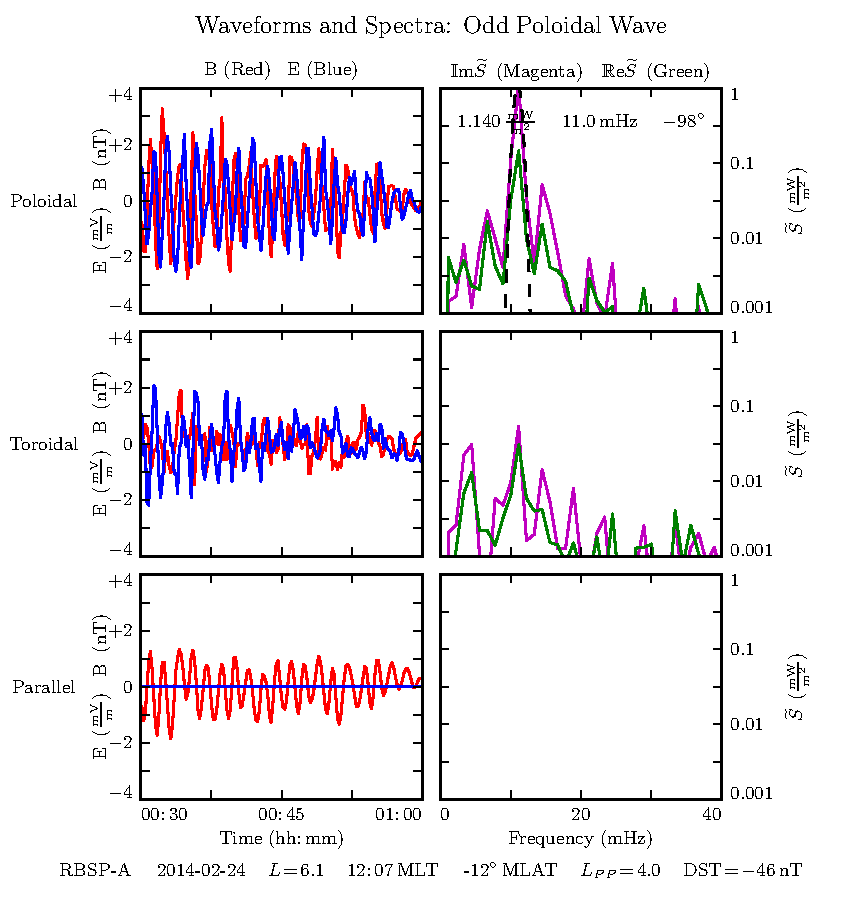
\includegraphics[width=\textwidth]{figures/sample_event_strong.pdf}
    \caption[Waveforms and Spectra for a Strong Pc4 Event]{
      \todo{$\cdots$}
    }
    \label{fig_sample_event_strong}
\end{figure}

\begin{figure}[!htb]
    \centering
    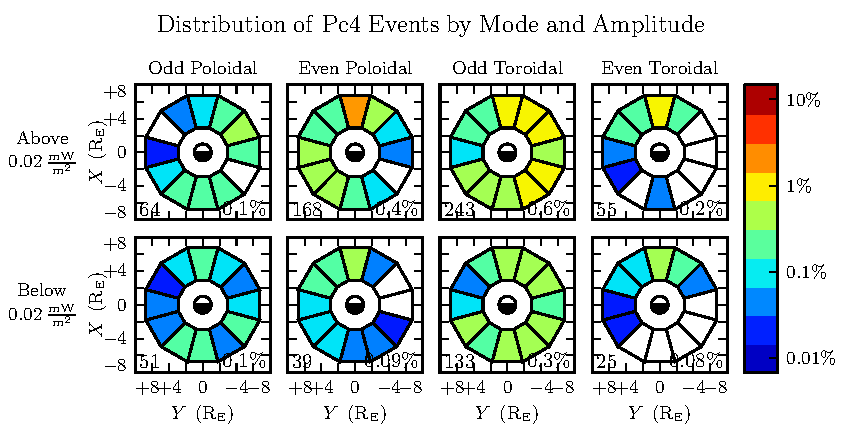
\includegraphics[width=\textwidth]{figures/mode_amp.pdf}
    \caption[Rate of Pc4 Events by Mode and Amplitude]{
      The above figure shows the distribution of Pc4 event observations by mode. Event magnitude cutoff is constant down each column, and increases from left to right. Stronger even events appear to become more concentrated on the dayside as the amplitude increases. Even poloidal events also become significantly more numerous relative to the other three modes, from \SI{26}{\percent} at a cutoff of \SI{0.01}{\mW/\m\squared} to \SI{41}{\percent} at \SI{0.1}{\mW/\m\squared}. 
    }
    \label{fig_mode_amp}
\end{figure}

% -----------------------------------------------------------------------------
% -----------------------------------------------------------------------------
% -----------------------------------------------------------------------------
\section{Events by Frequency}
  \label{sec_f}

The difference in magnetospheric conditions between the dayside and the nightside suggest that different eigenfrequencies should arise between dayside and nightside resonances at the same $L$-shell. In fact, this phenomenon has been observed directly; the frequencies of azimuthally-drifting FLRs have been shown to change over time\cite{motoba_2015}. The effect is attributed to the difference in mass loading (and thus \Alfven speed) as a function of MLT. 

This effect was furthermore apparent in the numerical results shown in \cref{ch_results}, where \Alfven speeds on the dayside (based on empirical profiles) gave rise to significantly higher eigenfrequencies than those on the nightside. 

In \cref{fig_mode_f}, events at \SIrange{11}{17}{\mHz} (center column) do seem to be shifted nightward compared to those at \SIrange{7}{11}{\mHz} (left column), but the effect is far more pronounced than what is suggested by \cref{sec_day,sec_night}. 

\todo{We should show the runs driven at $L\sim5$ across the board. Dayside and nightside. That way we can make a fair comparison. }

As might be expected, even events are more prevalent than first-harmonic-dominated odd events higher in the Pc4 range. Events at \SIrange{7}{11}{\mHz} (left column) outnumber those at \SIrange{17}{25}{\mHz} (right column) ten-to-one or more for odd events. Among even events, the comparison is closer to three-to-one. 

The spatial distribution of odd toroidal events above \SI{17}{\mHz} warrants specific consideration. Whereas odd toroidal events overall show an overwhelming preference for the morning side, those at the top of the Pc4 frequency band instead appear from noon to dusk. It's possible that this distribution is a consequence of the small number of events (25). More likely, however, is that these are third-harmonic events, and that their source more closely resembles the source for second-harmonic waves than it does first-harmonics. 

\todo{Have people looked at third harmonics? }

\begin{figure}[!htb]
    \centering
    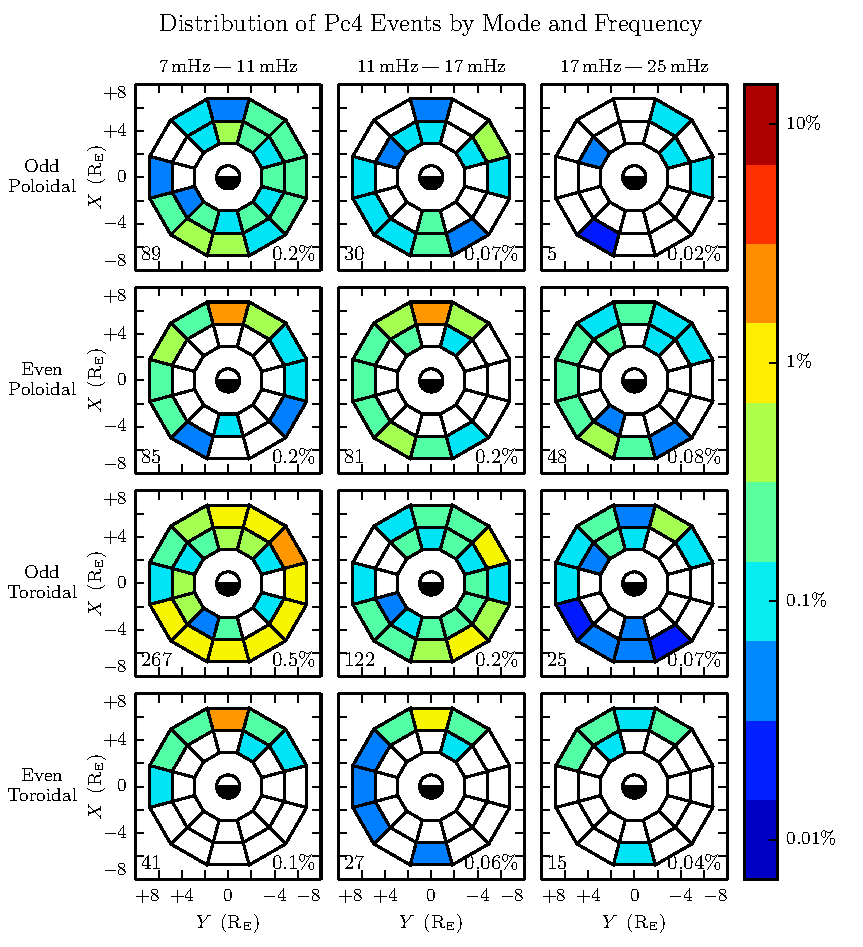
\includegraphics[width=\textwidth]{figures/mode_f.pdf}
    \caption[Rate of Pc4 Events by Mode and Frequency]{
      Event distributions above are shown in terms of mode (row) as well as event frequency (column). Mid-frequency Pc4 events are shifted somewhat nightward compared to low-frequency Pc4 events, as might be expected from the dayside's faster \Alfven speed. At the top of the Pc4 band, the distribution of odd toroidal events takes on a decidedly different character; this is likely because they are third harmonics rather than first harmonics. 
    }
    \label{fig_mode_f}
\end{figure}

The frequency distribution for each mode is shown in \cref{fig_f}. The most distinctive feature, certainly, is the frequency peak in the odd toroidal mode near \SI{9}{\mHz}. This is in line with the idea that toroidal waves exhibit frequencies that depend sharply on $L$, as discussed in \cref{ch_results}. While the Van Allen Probes' orbits do cover a large range of $L$-shells, their observations (and thus the selected events) are concentrated near apogee at $L \sim 6$. 

\begin{figure}[!htb]
    \centering
    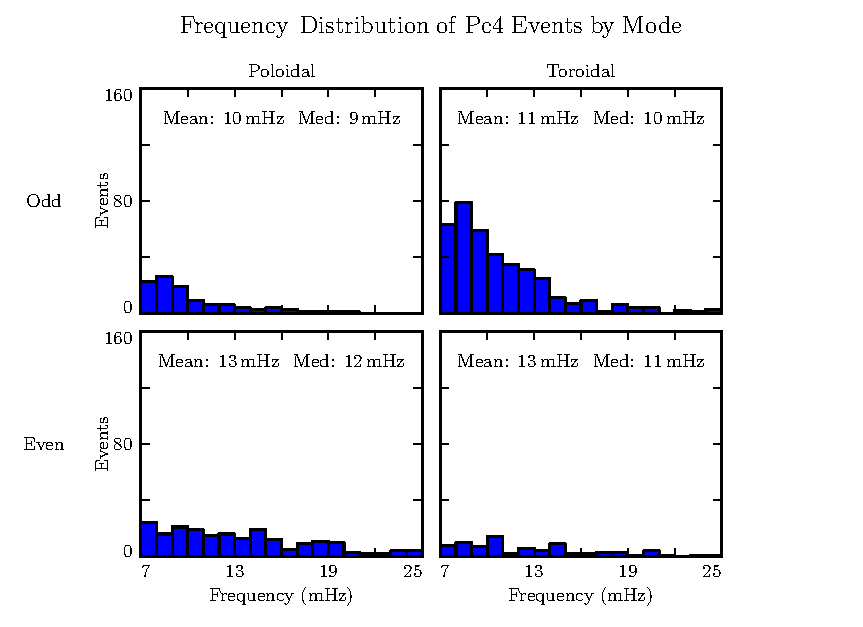
\includegraphics[width=\textwidth]{figures/f.pdf}
    \caption[Frequency Distribution of Pc4 Events by Mode]{
      Frequency distributions are shown for all events, divided by harmonic and polarization. Odd toroidal events exhibit a particularly sharp peak in frequency, which is consistent with the toroidal mode's strong correlation with the local eigenfrequency. Poloidal modes appear more spread out in frequency, which is also consistent with past observations and with the numerical results in \cref{ch_results}. 
    }
    \label{fig_f}
\end{figure}

\todo{Maybe put the Gaussian fit back on top of these distributions? The distributions are not particularly Gaussian, but it gives a quantitative estimate of the spread. }

% -----------------------------------------------------------------------------
% -----------------------------------------------------------------------------
% -----------------------------------------------------------------------------
\section{Events by Phase}
  \label{sec_phase}

The phase of a wave --- that is, the phase offset between a wave's electric and magnetic fields --- indicates how its energy is partitioned between the standing and traveling wave modes. An ideal standing wave has a phase of $\pm$\SI{90}{\degree}, and thus its Poynting flux is completely imaginary. A traveling wave, on the other hand, has electric and magnetic fields in phase (or in antiphase), and is associated with a net movement of energy, usually toward the ionosphere. 

Wave phase is a topic of significant interest, since it allows an estimate to be made of the wave's lifetime. And, because phase can only be determined using simultaneous electric and magnetic field measurements, it has only recently become observable. 

\todo{Do people really care about phase, or is it just John? }

The energy per unit volume, and the rate at which energy is carried out of that volume by Poynting flux, are respectively given by:
\begin{align}
  \label{def_phase}
  U &= \frac{R^3}{2\mz} B^2 &
  \ddt U &= \frac{R^2}{\mz} E B \cos\varphi
\end{align}

Where $B$, $E$, and $R$ are the characteristic magnetic field magnitude, electric field magnitude, and length scale. The phase, $\varphi \equiv \arctan\frac{ \imag\dft{S} }{ \real\dft{S} }$, enters because only real Poynting flux carries energy. 

The ratio of the two quantities in \cref{def_phase} gives a characteristic timescale over which energy leaves the system
\begin{align}
  \label{def_tau}
  \tau &\equiv \frac{BR}{2 E \cos\varphi}
\end{align}

In the present case, magnetic fields are on the order of \SI{1}{\nT} and electric fields are on the order of \SI{1}{\mV/\m}. A reasonable scale length might be \SI{e4}{\km}, the distance traversed by the probe over the course of a half-hour event (notably, back-to-back events are unusual). 

At a phase of \SI{80}{\degree}, this timescale is comparable to a Pc4 wave period. At \SI{135}{\degree}, where energy is divided evenly between the standing and traveling wave, the timescale is only 7 seconds. A wave with a phase so far from \SI{90}{\degree} would quickly vanish unless it were constantly being replenished. 

An example of just such an event is shown in \cref{fig_sample_event_phase}.  The left column shows electric and magnetic field waveforms in blue and red respectively. The right shows the corresponding spectra: imaginary Poynting flux in magenta (corrresponding to the strength of the standing wave) and real Poynting flux in green (for the traveling wave). The black line is a Gaussian fit to the magnitude of the Poynting flux. 

The poloidal channel shows a mostly-standing wave, with a phase of \SI{79}{\degree}. The coherent activity in the compressional magnetic field implies a low azimuthal modenumber, and thus a fast rotation of energy from the poloidal mode to the toroidal mode. It's likely the rotation of energy from the poloidal mode contributes significantly to the toroidal mode's lifetime; the toroidal wave's phase is \SI{130}{\degree}, so its energy should be carried away quickly by Poynting flux. 

\begin{figure}[!htb]
    \centering
    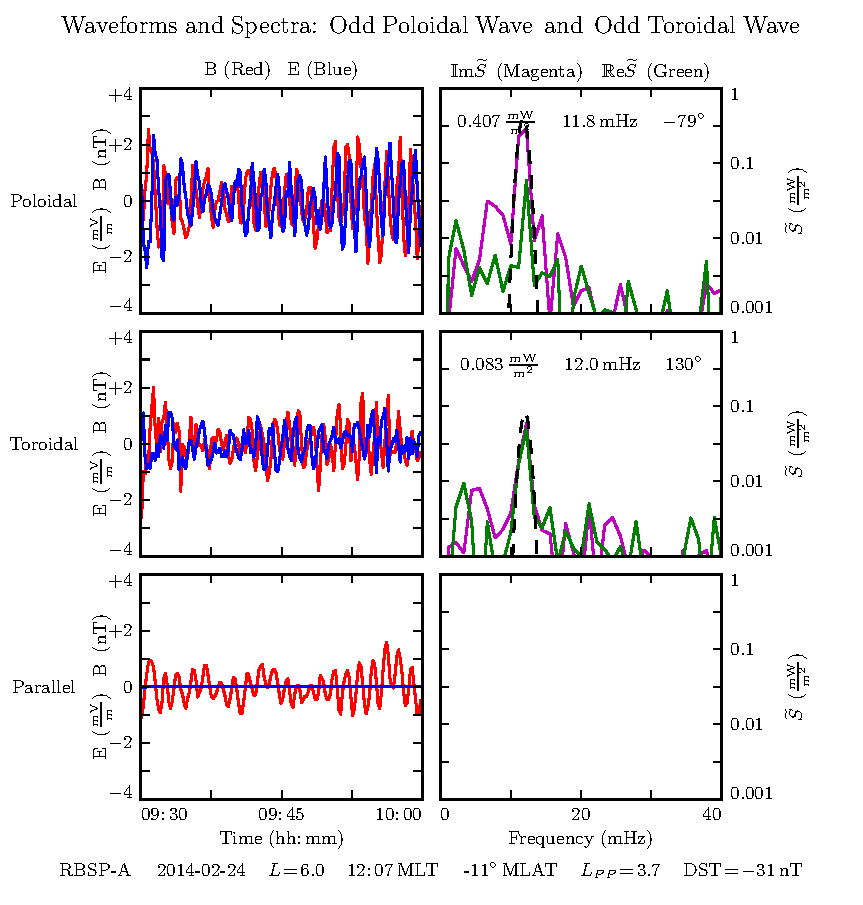
\includegraphics[width=\textwidth]{figures/sample_event_phase.pdf}
    \caption[Waveforms and Spectra for a Pc4 Event]{
      The above is a double event, where the poloidal and toroidal channels have been independently selected as events. The poloidal channel shows a wave with most of its energy in the standing wave (phase of \SI{79}{\degree}). The toroidal mode has a significant traveling component (phase of \SI{130}{\degree}). The compressional activity implies a low modenumber, which would cause energy to rotate quickly from the poloidal mode to the toroidal mode --- evidently at a sufficient rate to replenish the losses due to the traveling mode's real Poynting flux. 
    }
    \label{fig_sample_event_phase}
\end{figure}

The selection process described in \cref{sec_selection} does not explicitly consider phase. However, the discrete Fourier transform is performed over a half-hour time span. An event with a comparatively short lifetime would be unlikely to register. It's unsurprising to see the events in \cref{fig_phase}tightly clustered near \SI{90}{\degree}. 

\begin{figure}[!htb]
    \centering
    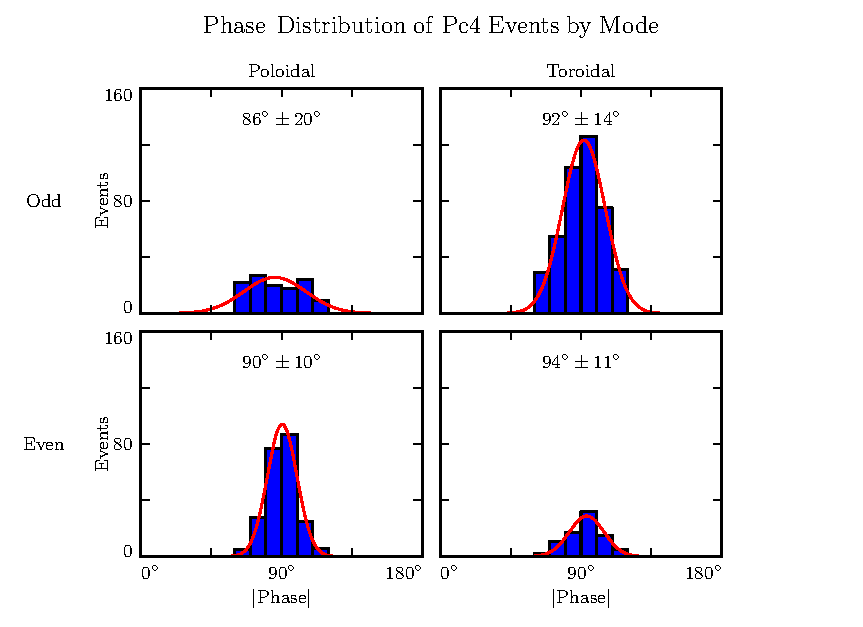
\includegraphics[width=\textwidth]{figures/phase.pdf}
    \caption[Phase Distribution of Pc4 Events by Mode]{
      The (absolute) phase of the selected Pc4 events is shown above. All modes show phase distributions peaked around \SI{90}{\degree}. This reflects the fact that a significant traveling wave component quickly carries energy away from an FLR. Odd events are spread more broadly in phase than even events. This is consistent with the odd modes' electric field antinode near the equator, where events are observed; the characteristic loss timescale depends on $\frac{B}{E}$ per \cref{def_tau}. 
    }
    \label{fig_phase}
\end{figure}

It's further notable in \cref{fig_phase} that the odd events are more spread out in phase than the even events. Near the equator, odd modes have an electric field antinode and a magnetic field node; per \cref{def_tau}, an odd mode's lifetime should be longer than that of an even mode with the same phase. \cref{fig_phase} uses the absolute value of each event's phase, as does \cref{fig_mode_phase}. 

Unlike amplitude (\cref{sec_amp}) and frequency (\cref{sec_f}), events of different phase do not seem to exhibit different spatial distributions, as shown in \cref{fig_mode_phase}. Comparisons are limited by the small event counts in several of the subplots; however, coarsely speaking, events with phases of \SI{75}{\degree} and worse (left column) show spatial distributions more or less in proportion with events phased \SI{85}{\degree} or better (right column). 

\begin{figure}[!htb]
    \centering
    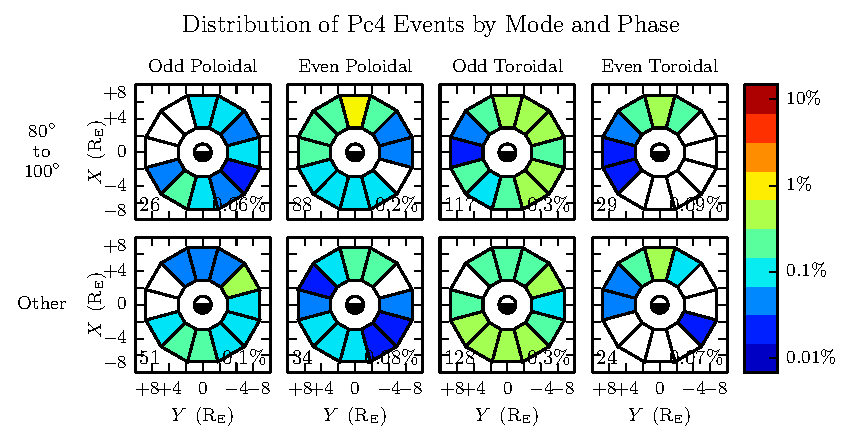
\includegraphics[width=\textwidth]{figures/mode_phase.pdf}
    \caption[Rate of Pc4 Events by Mode and Phase]{
      The observation rate of events is shown above, divided by (absolute) phase as well as mode. The closer a phase to \SI{90}{\degree}, the more of an event's energy is in the standing wave, rather than the traveling wave. The spatial distribution of events is more or less consistent between waves with phases very close to \SI{90}{\degree} and those with a significant traveling wave component. 
    }
    \label{fig_mode_phase}
\end{figure}

% -----------------------------------------------------------------------------
% -----------------------------------------------------------------------------
% -----------------------------------------------------------------------------
\section{Discussion}

\todo{Odd poloidal events and odd toroidal events are distributed similarly in space. Even poloidal events and even toroidal events too. Toroidal events are skewed dayward compared to poloidal events, which makes sense, since on the nightside poloidal-to-toroidal rotation timescales are comparable to dissipation timescales. }

\todo{Poloidal events are mostly even. Toroidal events are mostly odd. Maybe this indicates a different preference in modenumber? }

\todo{Even poloidal events are skewed toward high amplitude compared to the other modes. Stronger even poloidal events are also skewed dayward. }

\todo{Odd toroidal events near the top of the Pc4 frequency range exhibit qualitatively different behavior from the other odd toroidal modes. They are probably third harmonics. Maybe third harmonics have a source mechanism more like second harmonics than like first. }

\todo{Most events have (absolute) phase in the range \SIrange{80}{100}{\degree}, indicating that most of the energy is in the standing wave. Odd events are spread a bit more broadly in phase. This makes sense, since they ahve an electric field antinode near the equator (where measurements are made) which makes them less susceptible to energy loss from the traveling wave. }



% -----------------------------------------------------------------------------
% -----------------------------------------------------------------------------
% -----------------------------------------------------------------------------
%\section{Poloidal Pc4 Events by Compressional Coupling}

%\todo{Low-\azm poloidal Pc4 events are coupled to the compressional mode, while high-\azm ones are not. }

%\todo{The value of $\dft{B_z}/\dft{B_x} = 0.2$ comes from Dai\cite{dai_2015}. Can we match this up to an \azm value? Sounds like a job for Tuna! }

%\begin{figure}[!htb]
%    \centering
%    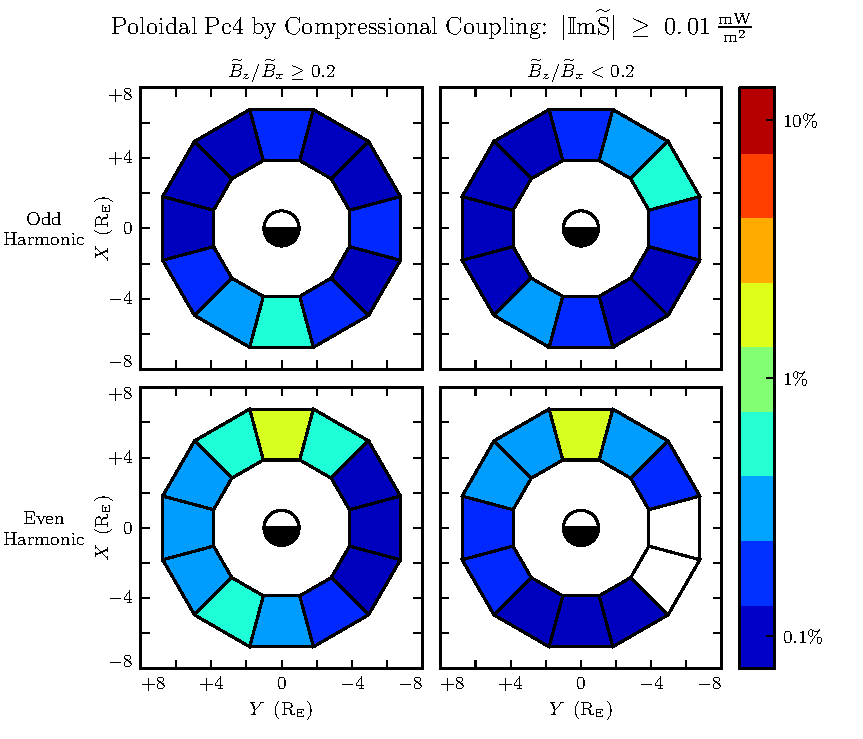
\includegraphics[width=\textwidth]{figures/azm_rate_all.pdf}
%    \caption[Poloidal Pc4 Rate by Compressional Coupling]{
%      \todo{Odd poloidal Pc4 events have a peak pre-noon and another peak near midnight. The pre-noon peak seems to be composed of high-\azm events, and the midnight peak seems to be low-\azm events. Low-\azm even poloidal events are spread broadly across the dusk side, while high-\azm even events are peaked strongly on the dayside --- consistent with Dai's results\cite{dai_2015}. }
%    }
%    \label{fig_azm_rate_all}
%\end{figure}




%\todo{Collections of events at a single ground observatory (near \SI{66}{\degree}) over significant periods of time: }

%Brekke\cite{brekke_1987} looked at 523 giant pulsation events recorded at Troms{\o}, Norway, from 1929 to 1985. This spanned several solar cycles. 

%Rolf\cite{rolf_1931} collected 28 events between 1921 and 1930 at Abisko. 

%Sucksdorf\cite{sucksdorff_1939} got 150 events between 1914 and 1938 in Sodankyl{\"a}. 

%Harang\cite{harang_1941}. 97 events from 1929 to 1941. Also Troms{\o}. Note that this may have been limited by the war! 

%This comes out to something like ... events over ... years. That's about ... giant pulsations per year, observed on the ground. 

%\todo{Collections of events at an array of ground observatories: }

%Chisham and Orr\cite{chisham_1991} found 34 events from 1984 to 1987 using the EISCAT magnetometer array in scandanavia. About \SI{5}{\degree} in MLT, decent coverage from \SIrange{63}{67}{\degree} mlat. This coincides with a solar minimum. 

%Motoba, in 2015, recorded 105 giant pulsation events. The observations were carried out by a number of ground magnetometers spanning $\sim \SI{90}{\degree}$ in local time and ranging roughly \SIrange{60}{70}{\degree} magnetic latitude\cite{motoba_2015}. This was mostly during a period of low solar activity, so we expect a high count. 

%\todo{Estimate of the size of an event's footprint:}

%Velkamp\cite{veldkamp_1960} looked at a single large event and showed that, at best, it was visible over a span of \SI{5}{\degree} in magnetic latitude. 

%This is seemingly consistent with the 29 February 2012 event discussed in detail by Motoba\cite{motoba_2015} --- Motoba shows some data, but doesn't discuss this aspect in detail. 

%Takahashi\cite{takahashi_2011} computes a FWHM of about 1 in L, or \SI{2}{\degree} magnetic latitude. 

%\todo{Tying that in to RBSP observations? }

%Note that it's a bit tricky to compare ground observations to in situ observations. Large-\azm events won't make it through the ionosphere. 

%There should be no bias with respect to MLT between a ground magnetometer and RBSP. Dai's analysis was specifically chosen to take advantage of the fact that RBSP's orbit had precessed all the way around the Earth. No preferred direction. And mlat shouldn't cause issues... these are FLRs, after all. 

%How strong does an event need to be on the ground, or in the sky, to count as a giant pulsation? Motoba 2015\cite{motoba_2015} has an event which tops out on the order of \SI{10}{\nT} on the ground. It's more like \SI{5}{\mV/\m} in situ. Takahashi\cite{takahashi_2011} has similar values. 

%If peak Pg observations are at $\SI{66}{\degree}$ mlat, that corresponds to $L = 6$. Then let's suppose that peak Pg viewing is $\SI{5}{\degree}$ wide --- estimating from the work of Velkamp and Motoba. That means RBSP should see lots of Pgs when it's between $L = 5.2$ andn $L = 7.1$. Well, \SI{7.1}{\RE} is outside its apogee, but the probes spend a fair amount of time outside $L = 5.2$, since they are moving pretty slowly at that point. 

%Giant pulsations have been shown to be more numerous in times of low solar activity. That was the whole point of Brekke's seminal 1987 paper, and it's consistent with what we show in \cref{ch_results}. The RBSP observations occur during peak solar times, though it's an anemic solar peak\cite{pesnell_2016}. 

%\todo{How much time does RBSP spend outside of $L = 5.2$ (for a range of \SI{5}{\degree})? How about $L = 5.6$ to $L = 6.5$ (for FWHM of \SI{2}{\degree}? }

%Each RBSP probe spends about \SI{30}{\percent} of its orbit between $L = 5.6$ and $L = 6.5$. 

%RBSP-A and RBSP-B count as two observers. In one $\sim 5$ cases out of hundreds do they simultaneously observe a poloidal Pc4 event (although, most notably for the 2012 event which \cite{dai_2013} considers in detail), both probes do fly through the same apparent event several hours apart from one another. 

%The duration of Dai's survey is October 2012 to June 2014. Scaled by 2 probes, each of which is present in the peak Pg lshells 30\% of the time, that comes out to almost exactly one year. 

%\todo{How many fundamental mode poloidal events do we see? How many could pass for giant pulsations? How many should we expect to see? }

%\todo{How weird is it for a fundamental mode poloidal Pc4 to be monochromatic? }

%\todo{How weird is it for a fundamental mode poloidal Pc4 to be stronger than \SI{5}{\mV/\m} at the equator? }











\chapter{Conclusion}
  \label{ch_conclusion}


% -----------------------------------------------------------------------------
% -----------------------------------------------------------------------------
% -----------------------------------------------------------------------------
\section{Summary of Results}

\todo{Write this. }


% -----------------------------------------------------------------------------
% -----------------------------------------------------------------------------
% -----------------------------------------------------------------------------
\section{Future Work}

Arbitrary deformation of grid. Get $\hat{e}_i = \frac{\partial}{\partial u^i} \underline{x}$, then $g_{ij} = \hat{e}_i \cdot \hat{e}_j$, then invert the metric tensor for contravariant components.  

MPI. Some benchmarks with time to compute vs time to broadcast. At what problem scale does additional parallelization make sense? 

Driving based on events? Wouldn't be that hard. 

Test particles? Seems silly. Watching something drift-bounce resonate will require making assumptions about what's going on on the other face of the planet.  

Conductivity affected by precipitation/current? 

IRI ionosphere model. Solar illumination effects. 


% Bibliography
\bibliography{thesis}

% Appendices
\appendix

%%%%%%%%%%%%%%%%%%%%%%%%%%%%%%%%%%%%%%%%%%%%%%%%%%%%%%%%%%%%%%%%%%%%%%%%%%%%%%%%
% app_glossary.tex: Glossary Appendix:
%%%%%%%%%%%%%%%%%%%%%%%%%%%%%%%%%%%%%%%%%%%%%%%%%%%%%%%%%%%%%%%%%%%%%%%%%%%%%%%%
\chapter{Glossary and Acronyms}
\label{app_glossary}
%%%%%%%%%%%%%%%%%%%%%%%%%%%%%%%%%%%%%%%%%%%%%%%%%%%%%%%%%%%%%%%%%%%%%%%%%%%%%%%%
Care has been taken in this thesis to minimize the use of jargon and
acronyms, but this cannot always be achieved.  This appendix defines
jargon terms in a glossary, and contains a table of acronyms and their
meaning.
%%%%%%%%%%%%%%%%%%%%%%%%%%%%%%%%%%%%%%%%%%%%%%%%%%%%%%%%%%%%%%%%%%%%%%%%%%%%%%%%

%%%%%%%%%%%%%%%%%%%%%%%%%%%%%%%%%%%%%%%%%%%%%%%%%%%%%%%%%%%%%%%%%%%%%%%%%%%%%%%%
% Glossary {{{
%%%%%%%%%%%%%%%%%%%%%%%%%%%%%%%%%%%%%%%%%%%%%%%%%%%%%%%%%%%%%%%%%%%%%%%%%%%%%%%%
\section{Glossary}
\label{jargonapp}
%%%%%%%%%%%%%%%%%%%%%%%%%%%%%%%%%%%%%%%%%%%%%%%%%%%%%%%%%%%%%%%%%%%%%%%%%%%%%%%%
\begin{itemize}

\item \textbf{Cosmic-Ray Muon} (\textbf{CR $\mu$}) -- A muon coming from
the abundant energetic particles originating outside of the Earth's
atmosphere.

\end{itemize}
%%%%%%%%%%%%%%%%%%%%%%%%%%%%%%%%%%%%%%%%%%%%%%%%%%%%%%%%%%%%%%%%%%%%%%%%%%%%%}}}

%%%%%%%%%%%%%%%%%%%%%%%%%%%%%%%%%%%%%%%%%%%%%%%%%%%%%%%%%%%%%%%%%%%%%%%%%%%%%%%%
% Acronyms {{{
%%%%%%%%%%%%%%%%%%%%%%%%%%%%%%%%%%%%%%%%%%%%%%%%%%%%%%%%%%%%%%%%%%%%%%%%%%%%%%%%
\section{Acronyms}
\label{acronymsec}
%%%%%%%%%%%%%%%%%%%%%%%%%%%%%%%%%%%%%%%%%%%%%%%%%%%%%%%%%%%%%%%%%%%%%%%%%%%%%%%%

% Table formatting

% Heading for the first page
\begin{longtable}{p{0.25\textwidth} p{0.75\textwidth}}
\caption{Acronyms} \label{tab:acronyms} \\

\toprule
Acronym & Meaning \\
\midrule
\endfirsthead

% Heading for all subsequent pages
\multicolumn{2}{l}{\textit{\tablename\ \thetable{} -- Continued from previous page}} \\
\toprule
Acronym & Meaning \\
\midrule
\endhead

% Footer for each page that wraps over to the next
\multicolumn{2}{r}{\textit{Continued on next page}} \\
\bottomrule
\endfoot

% Footer for the end of the table
\bottomrule
\endlastfoot

% End table formatting

CR$\mu$ & Cosmic-Ray Muon \\

\end{longtable}
%%%%%%%%%%%%%%%%%%%%%%%%%%%%%%%%%%%%%%%%%%%%%%%%%%%%%%%%%%%%%%%%%%%%%%%%%%%%%}}}


%% %%%%%%%%%%%%%%%%%%%%%%%%%%%%%%%%%%%%%%%%%%%%%%%%%%%%%%%%%%%%%%%%%%%%%%%%%%%%%
% %%%%%%%%%%%%%%%%%%%%%%%%%%%%%%%%%%%%%%%%%%%%%%% Appendix: Integrating Factors
% %%%%%%%%%%%%%%%%%%%%%%%%%%%%%%%%%%%%%%%%%%%%%%%%%%%%%%%%%%%%%%%%%%%%%%%%%%%%%








\chapter{Integrating Factors}
\label{app_integrating}

Start with differential equation of the form:

\begin{align}
  \frac{\partial}{\partial t} X(t) + \alpha X(t) &= \beta
\end{align}

Multiply by the integrating factor, then group terms: 

\begin{align}
  \exp (\alpha \; t) \frac{\partial}{\partial t} X(t) + \alpha \exp(\alpha \; t) X(t) &= \beta \exp(\alpha \; t) \\
  \frac{\partial}{\partial t} \big[ \exp(\alpha t) X(t) \big] &= \beta \exp(\alpha t)
\end{align}

Integrate from 0 to $\delta t$, assuming that $\beta$ is constant in time or varies slowly. 

\begin{align}
  \int^{\delta t}_0 dt \frac{\partial}{\partial t} \big[ \exp(\alpha t) X(t) \big] &= \int^{\delta t}_0 dt \beta \exp(\alpha t) \\
  \exp (\alpha \dt) X(\dt) - X(0) &= \dt \beta ( \frac{\dt}{2} ) \exp ( \alpha \frac{\dt}{2} )
\end{align}

Then rearrange to solve for the new value of X:

\begin{align}
  X(\delta t) &= X(0) \exp ( -\alpha \delta t ) + \delta t \beta ( \frac{\delta t}{2} ) \exp ( -\alpha \frac{\delta t}{2} )
\end{align}

Done. 


% End the Document
\end{document}




